% ==============================================================================
% RapidBoxForest (RBF) - IEEE Transactions on Robotics submission source (EN).
% Standalone-compilable from paper/ while reusing generated assets and figures
% from paper/generated/ and paper/figures/.
% ==============================================================================
% Load the silence package as early as possible to filter benign font warnings
% that are emitted during package/class loading in automated builds.
\RequirePackage{silence}
\WarningFilter{latexfont}{Font shape}
\WarningFilter{latexfont}{Some font shapes were not available}
\documentclass[journal]{IEEEtran}

% Font setup: keep the source portable across IEEE-style pdfLaTeX builds and
% XeLaTeX/LuaLaTeX builds.  For Unicode engines, load Latin Modern from TeX Live
% font files rather than relying on operating-system font discovery.
\usepackage{iftex}
\ifPDFTeX
  \usepackage[T1]{fontenc}
  \usepackage{lmodern}
\else
  \usepackage{fontspec}
  \setmainfont{lmroman10}[
    Extension=.otf,
    UprightFont=*-regular,
    BoldFont=*-bold,
    ItalicFont=*-italic,
    BoldItalicFont=*-bolditalic,
    Ligatures=TeX,
    Scale=MatchLowercase]
  \setsansfont{lmsans10}[
    Extension=.otf,
    UprightFont=*-regular,
    BoldFont=*-bold,
    ItalicFont=*-oblique,
    BoldItalicFont=*-boldoblique,
    Scale=MatchLowercase]
  \setmonofont{lmmono10}[
    Extension=.otf,
    UprightFont=*-regular,
    ItalicFont=*-italic,
    Scale=MatchLowercase]
\fi

% Loosen paragraph tolerance slightly to avoid underfull hbox warnings in
% narrow IEEE two-column layout while keeping good justification.
\tolerance=2000
\emergencystretch=2em
% Keep dense experiment floats near their discussion and let IEEE pages share
% more space between text and floats instead of creating float-heavy pages.
\setcounter{topnumber}{4}
\setcounter{dbltopnumber}{3}
\setcounter{bottomnumber}{3}
\setcounter{totalnumber}{6}
\renewcommand{\topfraction}{0.92}
\renewcommand{\bottomfraction}{0.80}
\renewcommand{\textfraction}{0.04}
\renewcommand{\floatpagefraction}{0.82}
\renewcommand{\dbltopfraction}{0.92}
\renewcommand{\dblfloatpagefraction}{0.82}
\setlength{\textfloatsep}{6pt plus 1pt minus 2pt}
\setlength{\dbltextfloatsep}{7pt plus 1pt minus 2pt}
\setlength{\floatsep}{5pt plus 1pt minus 2pt}
\setlength{\intextsep}{6pt plus 1pt minus 2pt}
\setlength{\abovecaptionskip}{3pt}
\setlength{\belowcaptionskip}{0pt}

\usepackage{amsmath,amssymb,amsfonts}
\usepackage{amsthm}
\usepackage{algorithm}
\usepackage{algorithmic}
\usepackage{booktabs}
\usepackage{array}
\usepackage{graphicx}
\usepackage{capt-of}
\usepackage{placeins}
\usepackage{bm}
\usepackage{cite}
\usepackage{hyperref}
\hypersetup{hidelinks}
\usepackage{cleveref}
\usepackage[inline]{enumitem}

\newtheorem{theorem}{Theorem}
\newtheorem{proposition}{Proposition}
\newtheorem{definition}{Definition}
\newtheorem{remark}{Remark}
\newtheorem{lemma}{Lemma}
\newtheorem{corollary}{Corollary}
\newtheorem{assumption}{Assumption}

\newcommand{\rbf}{RBF}
\newcommand{\iAABB}{\ensuremath{\mathrm{iAABB}}}
\newcommand{\Real}{\ensuremath{\mathbb{R}}}
\newcommand{\Ball}{\ensuremath{\mathbb{B}}}
\newcommand{\Cfree}{\ensuremath{\mathcal{C}_{\mathrm{free}}}}
\newcommand{\calO}{\ensuremath{\mathcal{O}}}
\newcommand{\Q}{\ensuremath{\mathcal{Q}}}
\newcommand{\cspace}{\mbox{C-space}}
\newcommand{\onlineq}{\mbox{Online/q}}
\newcommand{\Lref}{\ensuremath{L_{\mathrm{ref}}}}
\newcommand{\Lrefq}{\ensuremath{L_{\mathrm{ref},q}}}
\newcommand{\etal}{\textit{et al.}}
\renewcommand{\algorithmicrequire}{\textbf{Input:}}
\renewcommand{\algorithmicensure}{\textbf{Output:}}
\newcommand{\algcommentline}[1]{\STATE \textit{#1}}
\newcolumntype{L}[1]{>{\raggedright\arraybackslash}p{#1}}
\newcolumntype{M}[1]{>{\raggedright\arraybackslash}m{#1}}

% Keep table sizing local to each table or generated asset; avoid global font hooks
% that change IEEEtran table semantics. The restore macro is retained as a no-op
% for generated tables or earlier wrappers that may call it.
\newcommand{\TableFontRestore}{}

\begin{document}

\title{RapidBoxForest:\\ Certificate-Aware Box Reuse for Multi-Query Manipulation}

\author{Anonymous Authors%
\thanks{Submitted for double-anonymous review. Author affiliations and contact information are omitted from the review manuscript.}}

\maketitle

\begin{abstract}
Multi-query manipulation in semi-static workcells benefits from reusable
free-space structure, but existing reuse objects tend to be either edge-centric
roadmaps or expensive convex-region covers. RapidBoxForest (\rbf{}) introduces
a middle ground: a reusable forest of axis-aligned configuration-space
(\cspace{}) boxes validated by endpoint-to-link swept-capsule envelopes.
\rbf{} separates kinematics evidence from scene labels through a Lifelong
Envelope Cache Tree (LECT), recomputes obstacle labels for each scene, and uses
a typed corridor graph to distinguish certificate-backed regions from paths
that require fixed-step validation. Under saved Shelf+IIWA
catalogs and a common 8-thread policy, a prebuilt depth-23 LECT cache gives
0.171~s median reusable build time and 0.077~s median per-query online time,
versus 2.770~s live HIFK-5 build time. Across random-scene catalogs on three
robot models, \rbf{} trades some RRT-Connect per-query speed for shorter
validated paths and lower online time than BIT*. Local edit experiments report
maintenance-only cache-update speedups of 153.3--207.5$\times$ for insertion
and 943.6--3354.0$\times$ for removal over a 15-obstacle warm rebuild.
\end{abstract}

\begin{IEEEkeywords}
Motion planning, manipulation planning, multi-query planning, collision checking,
configuration-space decomposition, link envelopes.
\end{IEEEkeywords}

\begin{table*}[!t]
\centering
\caption{Reusable state in planning paradigms. \rbf{} is positioned as
low-overhead volumetric reuse with explicit returned-path semantics.}
\label{tab:related_qualitative_comparison}
\footnotesize
\setlength{\tabcolsep}{2.6pt}
\renewcommand{\arraystretch}{1.10}
\begin{tabular}{@{}M{0.18\textwidth}M{0.18\textwidth}cM{0.25\textwidth}M{0.26\textwidth}@{}}
\toprule
Paradigm family & Reused state & Vol. & Update or validation style & Multi-query implication \\
\midrule
Roadmap reuse (PRM/LazyPRM) & Vertices, edges, and cached edge checks & No & Recheck affected edges after scene changes & Strong graph reuse, but no reusable free-volume unit. \\
Tree and anytime sampling (RRT, RRT-Connect, BIT*, FMT*) & Query tree or batch sample graph & No & Primarily query-local; rebuilt or checkpointed & Fast discovery or quality improvement without persistent volumetric scene structure. \\
Convex-region optimization (IRIS/GCS) & Convex cells and region graph & Yes & Inflate, certify, or recertify regions after edits & Optimization-ready regions, but update cost can dominate short query batches. \\
\rbf{} & Box forest, typed graph, and LECT evidence & Yes & Recheck boxes, replay kinematics evidence, and validate non-certificate outputs & Low-overhead free-volume reuse with auditable certificate boundaries. \\
\bottomrule
\end{tabular}
\end{table*}



% ==============================================================================
\section{Introduction}\label{sec:intro}

Many high-degree-of-freedom manipulation systems solve streams of related
queries in nearly fixed workcells. Robot kinematics persist, while start--goal
pairs, local obstacles, and small scene edits change. This pattern appears in
machine tending, shelf transfer, inspection, and pick-and-place cells, where the
robot model is fixed but clutter and requested endpoints vary across a shift. A
useful reusable object for this setting should therefore do more than store a
previous path: it should accelerate later queries, remain cheap to update, and
state clearly which parts of a returned path are certified.

Existing reuse mechanisms tend to emphasize one side of this trade-off.
Sampling-based planners and roadmap variants reuse vertices, edges, or prior
paths~\cite{lavalle2006planning,lavalle1998rapidly,kavraki1996probabilistic,
karaman2011sampling}, but the reused object is usually non-volumetric.
Convex-region methods such as Iterative Regional Inflation (IRIS) and Graphs of
Convex Sets (GCS) provide optimization-ready free-space regions~\cite{
deits2015computing,marcucci2023motion,marcucci2024shortest}, but their regions
can be expensive to construct, certify, and repair after edits.

RapidBoxForest (\rbf{}) targets the middle ground. It grows reusable
axis-aligned configuration-space (\cspace{}) boxes around scene-relevant seeds,
validates them with endpoint-to-link swept-capsule envelopes, and connects
accepted boxes in a typed corridor graph. The boxes are not the tightest possible
\cspace{} regions; they are chosen because replay, adjacency, invalidation, and
local repair remain simple enough to expose directly.

\paragraph{Problem statement}
Let $\Q\subset\Real^n$ be the joint-limit box of a fixed
\(n\)-degree-of-freedom manipulator and let $\calO\subset\Real^3$ be the
current workspace obstacle set. Given a set or stream of start--goal queries
$(q_s,q_g)\in\Q^2$, \rbf{} constructs a finite family of \cspace{} boxes that
pass the configured scene-validation policy and uses those boxes as vertices of
an adjacency graph. The design target is a query-agnostic, volumetric, and
auditable scene structure, not an exhaustive decomposition of $\Cfree$.

\paragraph{Key idea and terminology preview}
The geometric identity behind the method is classical: if the endpoint sweeps of
a rounded link are bounded, then the link sweep is bounded by the convex hull of
those endpoint bounds plus the link radius. The contribution is to use this
identity as a reusable \cspace{} box validator. Three semantic layers are used
throughout the paper: \emph{geometry evidence} denotes obstacle-independent
endpoint and link envelopes stored in LECT; \emph{scene structure} denotes the
current boxes, labels, and typed graph edges recomputed after obstacle checks;
and \emph{returned-path status} is certificate-backed only inside conservative
regions and otherwise validation-required. The unified guarantee matrix appears
in \Cref{tab:claim_boundary} after the collision model is defined.

This paper makes three contributions.
\begin{enumerate}[nosep,leftmargin=*]
  \item \emph{A conservative box-region certificate primitive.}
  Endpoint-to-link swept-capsule bounds convert endpoint envelopes into link
  envelopes over a \cspace{} box, giving a reusable collision-free box
  certificate when the endpoint source, radius padding, and separation tests are
  conservative. This gives the planner a reusable free-volume unit rather than
  only checked edges.
  \item \emph{A certificate-aware reusable box-forest planner.}
  \rbf{} grows policy-accepted \cspace{} boxes, assembles them into a scene
  forest and typed corridor graph, and exposes whether a returned segment is
  certificate-backed or validation-required. This lets the query interface make
  returned-path semantics explicit instead of hiding them inside post hoc checks.
  \item \emph{A two-level reuse and maintenance architecture.}
  LECT indexes robot-kinematic envelope records separately from scene labels;
  the scene cache handles local obstacle insertions and deletions by rechecking
  affected boxes and replaying compatible geometry evidence. This separates
  kinematic reuse from scene relabeling, which makes local edits cheaper and
  easier to audit.
\end{enumerate}
The experiments are therefore organized around these semantics: reusable build
cost, online query time, validation responsibility, and edit maintenance are
reported separately.

Fig.~\ref{fig:linkiaabb} summarizes the method framework: link-interval
computation produces reusable geometry evidence, \rbf{} growth recomputes scene
labels and graph connectivity for the current obstacles, and LECT replay changes
construction cost without changing validation responsibility.
Sections~\ref{sec:link_envelopes}--\ref{sec:exp} make these blocks precise and
then evaluate them.

\begin{figure*}[!t]
\centering
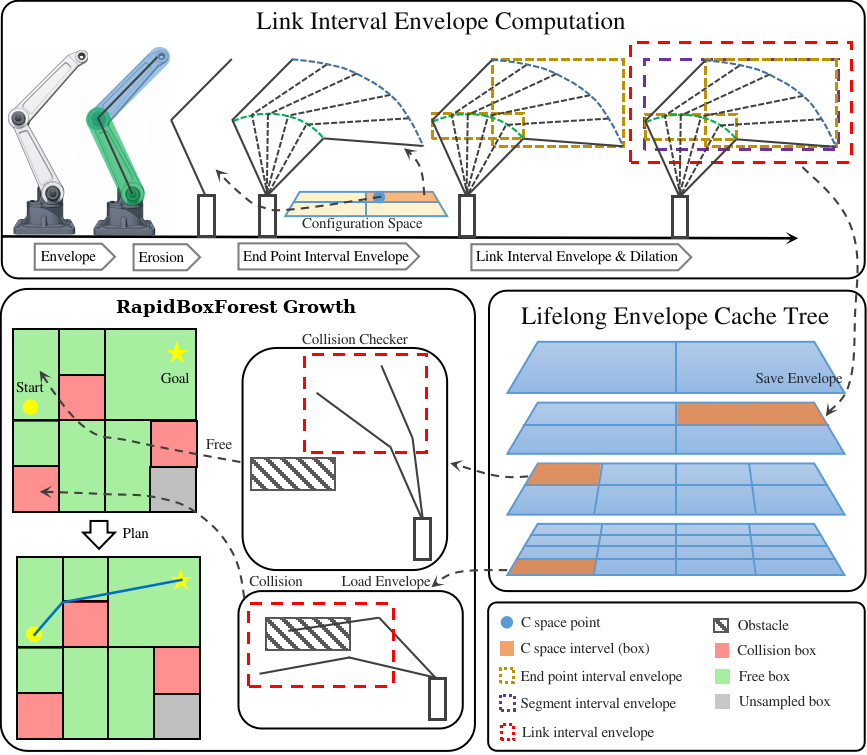
\includegraphics[width=0.94\textwidth]{figures/framework.png}
\caption{\rbf{} pipeline. Top: endpoint and segment interval envelopes induce
link interval envelopes over a \cspace{} interval. Lower left: sample-guided
\rbf{} growth labels free, collision, and unsampled boxes. Lower right: LECT
stores kinematics-keyed envelope records for replay. Reused: geometry evidence.
Recomputed: obstacle labels and graph edges. Accepted outputs: conservative
corridors or paths accepted after fixed-step validation.}
\label{fig:linkiaabb}
\end{figure*}

% ==============================================================================
\section{Related Work}\label{sec:related}

Region-based planners make collision-free volume an explicit planning object.
IRIS variants inflate collision-free convex regions, and Graphs of Convex Sets
(GCS) optimize over the induced region graph~\cite{deits2015computing,
marcucci2023motion,marcucci2024shortest,amice2022finding,
petersen2023growing,werner2024approximating}. \rbf{} shares the goal of
reusing free volume but uses axis-aligned \cspace{} boxes rather than arbitrary
convex cells, explicitly trading expressivity for cheaper local validation,
adjacency, cache replay, and maintenance. \Cref{tab:related_qualitative_comparison}
is therefore not only a taxonomy: it identifies the gap targeted here, namely low-overhead
volumetric reuse between roadmap reuse and optimization-ready convex covers.

\noindent\emph{Synthesis.}
Existing reuse objects are either cheap but edge-centric, or volumetric but
costly to construct and repair. \rbf{} is not intended to dominate either class
universally. Its intended niche is repeated manipulation in scenes where a
volumetric reusable layer is valuable, but repeatedly inflating optimization-ready
convex regions or rebuilding large roadmaps is too expensive for local edits and
short query batches.

\paragraph{Continuous-collision-detection endpoint bounds}
\label{sec:related_endpoint_bounds}
Swept-volume and interval-kinematics methods supply the geometric primitives
used here. Convex-hull generator bounds and capsule radius lifts provide
swept-set enclosures, while the Proximity Query Package (PQP),
Gilbert--Johnson--Keerthi (GJK), the Flexible Collision Library (FCL), and
interval Denavit--Hartenberg propagation provide collision-query and
interval-kinematics primitives used in related continuous-collision-detection
pipelines~\cite{blackmore1992swept,abdel2006swept,
gottschalk1996obbtree,larsen1999fast,gilbert1988fast,bergen1999gjk,
pan2012fcl,moore2009introduction,jaulin2001applied,snyder1992interval,
merlet2004solving,merlet2009interval}. Redon \etal{} combine such primitives for
articulated-body continuous collision detection over time
steps~\cite{redon2004ccd_avatar,redon2005fast_artic}; related Taylor-model and
safety methods use similar swept-sphere
bounds~\cite{zhang2007taylor,schwarzer2005adaptive,corrales2011ssl}. The
novelty in \rbf{} is not the endpoint bound alone, but its use as a reusable
joint-box validator: compatible evidence is stored in LECT, replayed before
scene-specific obstacle tests, and interpreted through the claim boundary in
\Cref{tab:claim_boundary}.

\paragraph{Graph reuse}
Reusable graph planners amortize effort across related queries. Probabilistic
roadmaps (PRMs) and LazyPRM reuse roadmaps and edge checks~\cite{kavraki1996probabilistic,bohlin2000path,
dellin2016unifying,schmerling2015optimal}, experience-based systems reuse prior
paths~\cite{coleman2014moveit}, and adaptive cell methods split cells until
they obtain a searchable accepted-cell graph~\cite{lozanoperez1983spatial,
brooks1985subdivision}. \rbf{} keeps the multi-query graph-search benefit but
changes the reused unit: vertices are accepted free-volume boxes, edges are
typed by certificate status, and kinematics evidence is separated from scene
labels rather than saved as stale obstacle outcomes.

\paragraph{Sampling and refinement}
Rapidly-exploring random tree (RRT) variants, Batch Informed Trees (BIT*),
Fast Marching Tree (FMT*), and the Open Motion Planning Library (OMPL) provide
standard single-query planners, anytime references, and benchmarking
infrastructure~\cite{karaman2011sampling,kuffner2000rrt,
gammell2015batch,gammell2018informed,janson2015fmt,sucan2012ompl,
moll2015benchmarking}. Trajectory optimizers refine supplied
paths~\cite{ratliff2009chomp,kalakrishnan2011stomp,schulman2014motion,
mukadam2018gpmp2}. \rbf{} is therefore not positioned as a single-query optimal planner;
it supplies reusable volumetric context before repair, shortcutting,
optimization, and final fixed-step validation.

% ==============================================================================
\section{Link Interval Envelopes}\label{sec:link_envelopes}

This section defines the geometric certificate primitive used later. The
link-envelope validation layer maps joint regions to endpoint and link bounds;
graph connectivity and query acceptance are handled by later layers. For a
joint region
$I\subseteq\Q$, endpoint envelopes $E_k(I)$ bound endpoint trajectories for
endpoint $k$, and link envelopes $B_\ell(I)$ bound rounded links for link
$\ell$ over the same region:
\[
I \mapsto \{E_k(I)\} \mapsto \{B_\ell(I)\}.
\]
Axis-aligned \cspace{} boxes are the default regions; local oriented bounding
boxes (OBBs) in scaled joint coordinates appear only as typed bridge corridors.
Endpoint evidence becomes a certificate only after it is lifted to link
envelopes and those envelopes pass conservative scene-separation tests. All
empirical or otherwise non-conservative endpoint sources are treated as filters
under \Cref{tab:claim_boundary}.

\begin{samepage}
\begin{assumption}[Collision model for certificates]
\label{ass:collision_model}
The certificate model covers only workspace-obstacle collision between active
rounded links and $\mathcal{O}$; joint limits are enforced separately by
requiring $I\subseteq\Q$.
Self-collision, attachments, grippers, task regions, and other constraints are
outside this certificate model unless encoded in the validation policy and cache
descriptor. The experiments instantiate this subset with active-link
versus workspace-obstacle collision checks.
\end{assumption}
\end{samepage}

\begin{table*}[!t]
\centering
\caption{Guarantee matrix for returned objects. Status is interpreted under
\Cref{ass:collision_model} and the experiment protocol in \Cref{sec:exp}.}
\label{tab:claim_boundary}
\footnotesize
\setlength{\tabcolsep}{3.0pt}
\renewcommand{\arraystretch}{1.10}
\begin{tabular}{@{}M{0.26\textwidth}M{0.18\textwidth}M{0.48\textwidth}@{}}
\toprule
Object or state & Status & Condition \\
\midrule
Path inside conservative box union & Certificate-backed & Every traversed box passes conservative endpoint-to-link validation against the current obstacles. \\
Path inside finite-cover OBB corridor & Certificate-backed & Every cover tile in the local \cspace{} OBB corridor passes the same box test. \\
Gap, segment, or repair witness & Validation-required & Certificate-backed only after conversion to a conservative box or OBB corridor. \\
Filter-derived path & Validation-required & Empirical or non-conservative evidence may guide planning but cannot certify coupled extrema. \\
LECT replay record & No path claim & Reuses descriptor-compatible geometry evidence only; scene labels and graph edges are recomputed. \\
\bottomrule
\end{tabular}
\end{table*}

\noindent\emph{Reporting convention.}
A certificate-backed object is collision-free under \Cref{ass:collision_model}; a
validation-required object may guide planning but becomes an accepted path only
after the fixed-step validation protocol in \Cref{sec:exp}. Cache hits change
construction cost, not validation responsibility. Planning aids that are not
certificate-backed follow the semantics in \Cref{tab:claim_boundary}.
Shortcutting or simplification inherits a certificate only when containment
inside the certified region is preserved; otherwise it follows the
validation-required semantics in \Cref{tab:claim_boundary}. Timing claims using
\onlineq{} refer to planner online time rather than total accepted-path wall
clock unless an additional validation or simplification cost is explicitly
reported. Compact tables without audit-cost columns therefore do not support
total-latency comparisons.

\subsection{Geometric Foundation}\label{sec:rewrite_geom}

Let \(C_0\) be a body-frame shape. The rigid transform
$T(q)x=R(q)x+t(q)$ maps a body-frame point \(x\) to workspace at configuration
$q$, with rotation $R(q)$ and translation $t(q)$, and
$\mathcal{S}_I(C_0)$ denotes the workspace set swept by \(C_0\) as $q$ ranges
over $I$. Let \(\Ball_p(r)\) denote the radius-\(r\) ball in the \(p\)-norm, and
let \(\oplus\) denote Minkowski sum. For a capsule $C=S\oplus \Ball_2(r)$ with
zero-radius center segment \(S\), the fixed-radius ball commutes with rigid
motion:
\[
\mathcal{S}_I(C)=\mathcal{S}_I(S)\oplus \Ball_2(r).
\]
Thus a rounded link can be bounded by first bounding the zero-radius center
segment and then lifting by the link radius. For a convex body
$P=\operatorname{conv}(v_1,\ldots,v_m)$ with vertices \(v_i\), outer bounds on
the vertex trajectories also bound the swept body,
\[
\mathcal{S}_I(P)\subseteq
\operatorname{conv}\Bigl(\bigcup_{i=1}^{m} \widehat{\Gamma}_i(I)\Bigr).
\]
Here \(\widehat{\Gamma}_i(I)\) denotes a conservative outer bound on the
workspace trajectory of vertex \(v_i\), \(i=1,\ldots,m\), over \(I\).
For a capsule link, only the two endpoint trajectories are needed. Let
\(\Gamma_a(I)\) and \(\Gamma_b(I)\) denote the exact workspace trajectories of
the proximal and distal endpoints over \(I\). \rbf{} uses these swept-sphere
bounds over a configuration-space box domain and stores the resulting bounds as
reusable kinematics-keyed bound records.

\begin{samepage}
\begin{proposition}[Endpoint envelopes induce link interval envelopes]
\label{prop:endpoint_to_link_envelope}
Consider a rounded link $L=[a,b]\oplus \Ball_2(r)$ and a joint interval $I$. If
endpoint envelopes $E_a(I)$ and $E_b(I)$ satisfy
$\Gamma_a(I)\subseteq E_a(I)$ and $\Gamma_b(I)\subseteq E_b(I)$, then
\[
\mathcal{S}_I(L)
\subseteq
\operatorname{conv}\bigl(E_a(I)\cup E_b(I)\bigr)\oplus \Ball_2(r).
\]
Consequently, any conservative outer representation of the right-hand side is a
valid link interval envelope for the whole joint interval $I$.
\end{proposition}
\end{samepage}

\begin{proof}
For each $q\in I$, the center segment of the moved link is the convex hull of
the two moved endpoints, and those endpoints lie in
\(\Gamma_a(I)\) and \(\Gamma_b(I)\). Hence all center segments are contained in
\(\operatorname{conv}(\Gamma_a(I)\cup\Gamma_b(I))\). The endpoint inclusions
place this set inside \(\operatorname{conv}(E_a(I)\cup E_b(I))\). Adding the
fixed radius ball commutes with the rigid-motion sweep of the capsule, giving
the stated containment.
\end{proof}

\begin{corollary}[Conservative configuration-space box validation]
\label{cor:box_validation}
Let $I\subseteq\Q$ be an axis-aligned configuration-space box and let
$\{B_\ell(I)\}$ be conservative link interval envelopes for all active rounded links. If
$B_\ell(I)\cap\calO=\emptyset$ for every link $\ell$, then every configuration
$q\in I$ is collision-free with respect to the collision model in
\Cref{ass:collision_model}.
\end{corollary}

\begin{proof}
By \Cref{prop:endpoint_to_link_envelope}, each conservative link envelope
contains the swept workspace volume of its link over all configurations in
$I$. This disjointness from $\calO$ for every active link excludes workspace
obstacle collision for the whole manipulator at every $q\in I$ under
\Cref{ass:collision_model}.
\end{proof}

\paragraph{Numerical conservatism}
A certificate is claimed only when endpoint propagation, radius padding, and
obstacle separation produce outward bounds under the collision model of
\Cref{ass:collision_model}. For link radius \(r_\ell\), the axis-aligned
bounding box (AABB) broadphase pads by the infinity-norm ball
\(\Ball_\infty(r_\ell)\), which conservatively contains the Euclidean radius
lift \(\Ball_2(r_\ell)\). SupportHull/GJK denotes a
support-function hull with GJK refinement; it is certificate-backed only with
outward obstacle inflation, explicit margins, and conservative termination
tolerances. Empirical endpoint sources and post-processing outside a
conservative box union or a finite-cover OBB-corridor union are treated as
non-conservative filters; they do not extend \Cref{cor:box_validation} or
\Cref{lem:corridor_certificate}.

\subsection{Endpoint Interval Envelopes}\label{sec:rewrite_endpoint_env}

For endpoint $k$, let $\Gamma_k(I)$ be its exact trajectory over joint interval
$I$.
Any conservative set containing $\Gamma_k(I)$ is an endpoint interval envelope;
the basic record is an endpoint axis-aligned bounding box (AABB) because it is
compact and directly reusable by all link-envelope representations. Two
certificate-backed endpoint sources are used. Interval forward kinematics (IFK)
denotes the unsplit interval pass; \mbox{IFK-AA} is the affine-arithmetic
implementation that propagates bounds along the Denavit--Hartenberg chain, with
shared noise symbols preserving part of the trigonometric correlation.
Hierarchical IFK (HIFK) bisects the joint interval and forms hulls of child
endpoint boxes, reducing wrapping at higher materialization cost. HIFK is a
hierarchical split-and-hull evaluation
(for example, \mbox{HIFK-5} means five split levels), so the split depth is part
of the cache descriptor and cannot be exchanged with an unsplit record. A
critical-sample source probes interval endpoints,
midpoints, near-boundary configurations, and trigonometric turning candidates;
it can reduce over-approximation relative to IFK, but does not certify coupled
extrema.
An analytical extrema source solves low-dimensional sinusoidal boundary
subproblems, reducing one- and two-joint boundary cases to structured root
search. It becomes conservative only with an interval-closure wrapper; the
Analytical row in Table~\ref{tab:tro-endpoint-envelope} is otherwise a
comparison reference.
Without such a wrapper, critical-sample and analytical endpoint sources are
filters rather than certificate evidence. Any path using either source is
accepted only after fixed-step validation unless wrapped by an independent
conservative certificate. During LECT tree descent, transient prefix transforms are reused so
unaffected kinematic-chain prefixes are not recomputed. This affects runtime
materialization only; it is not persistent scene state.
The upper panel of Fig.~\ref{fig:linkiaabb} summarizes this endpoint-to-link
conversion before the scene check accepts a box.

\subsection{C-space OBB Endpoint Envelopes}\label{sec:obb_endpoint_env}

Axis-aligned boxes remain the global forest primitive. Bridge and repair motions
introduce local joint correlations. For a bridge transition to carry a
certificate, \rbf{} validates a local typed \cspace{} \mbox{OBB-corridor}
region with the finite-cover test below, while leaving the dyadic forest
unchanged. Without a successful finite cover, the same transition remains only a
typed candidate that requires fixed-step validation. OBBs are defined
in scaled joint coordinates. Let \(q_c\) be the local corridor center, and let
\(S\in\Real^{n\times n}\) be a diagonal joint-scaling matrix with positive
diagonal entries, defining the local metric. Let \(m\le n\) be the local dimension,
\(U\in\Real^{n\times m}\) have scaled-metric orthonormal columns, and
\(h\in\Real_{\ge 0}^{m}\) be the half-width vector. With the local cube
\(\Xi=\{\xi\in\Real^m\mid -1\le \xi_i\le 1,\ i=1,\ldots,m\}\) and
\(A=S^{-1}U\operatorname{diag}(h)\in\Real^{n\times m}\),
the local region is
\[
R_{\mathrm{obb}}
=
\{\,q_c + A\xi \mid \xi\in\Xi\,\}.
\]
The object \(R_{\mathrm{obb}}\) is a configuration-space region, not a workspace OBB:
the certificate comes from endpoint and link envelopes over \(R_{\mathrm{obb}}\), not
from the fitted orientation.

\paragraph{Cover certificate}
The conservative cover test tiles the local cube into subcubes \(X_\tau\), where
\(\tau\) indexes the cover tiles; for each \(X_\tau\subseteq\Xi\), it forms the
joint-space AABB hull
\[
I_\tau=\operatorname{bbox}_q(q_c+A X_\tau),
\]
where \(\operatorname{bbox}_q(\cdot)\) denotes the joint-space AABB hull. If
every \(I_\tau\) passes the standard conservative link-envelope scene test, then
\[
R_{\mathrm{obb}}\subseteq \bigcup_\tau I_\tau \subseteq \Cfree,
\]
where \(\Cfree\) is the collision-free configuration set under
\Cref{ass:collision_model}. When this test succeeds, the stored OBB certificate
is a finite cover of axis-aligned box certificates.

\paragraph{Correlated endpoint envelope}
A tighter source keeps the local OBB variables \(\xi\) correlated through the
forward-kinematics computation. For each joint coordinate \(j=1,\ldots,n\),
\[
q_j=q_{c,j}+a_j^\top\xi,\qquad \xi_i\in[-1,1],\ i=1,\ldots,m,
\]
where \(a_j^\top\) is the \(j\)-th row of \(A\). Affine-arithmetic propagation
then produces endpoint records with center \(c_k\), generators \(g_{k,i}\), unit
noise variables \(\epsilon_i\in[-1,1]\), and a coordinatewise nonnegative
remainder vector \(\rho_k\):
\[
E_k(R_{\mathrm{obb}})
=
c_k+\sum_i g_{k,i}\epsilon_i \oplus [-\rho_k,\rho_k].
\]
The sum runs over the affine-noise generators in the endpoint record.
Equivalently, with \(p_k(q_c)\) the endpoint position and \(J_k(q_c)\) its
Jacobian at the corridor center,
\[
E_k(R_{\mathrm{obb}})
=
p_k(q_c)+J_k(q_c)A\Xi \oplus [-\rho_k,\rho_k],
\]
\begin{samepage}
where \(\mu\in\{1,2,3\}\) indexes workspace coordinates, the sum is over local
coordinates \(a,b=1,\ldots,m\), and each coordinate remainder is bounded
conservatively, for example by
\[
\rho_{k,\mu}\ge
\frac{1}{2}\sum_{a,b}
\left|{\left(A^\top H_{k,\mu}A\right)}_{ab}\right|,
\]
with \(H_{k,\mu}\) an interval or otherwise conservative Hessian bound over
\(R_{\mathrm{obb}}\). If these remainders are sampled rather than outward bounded,
the OBB source is a non-conservative filter and not a certificate.
\end{samepage}

OBB endpoint records feed the same endpoint-to-link construction as axis-aligned
\cspace{} boxes.
These records refine a local typed edge; they do not add OBB nodes to the global
axis-aligned forest.
For a workspace support direction \(d\in\mathbb{R}^3\), the support function of
a zonotope-plus-box endpoint record is
\[
h_{E_k}(d)=d^\top c_k+\sum_i |d^\top g_{k,i}|
          +\sum_{\mu=1}^3 |d_\mu|\rho_{k,\mu}.
\]
Here the sum over \(i\) spans the affine-noise generators in the
endpoint record, and \(\mu\) indexes workspace coordinates.
Because \(E_a\) and \(E_b\) enclose the endpoint trajectories, a conservative
support bound for the zero-radius link centerline is
\[
\bar h_\ell^\circ(d)=\max\{h_{E_a}(d),h_{E_b}(d)\},
\]
and radius lifting gives the rounded-link support bound
\[
\bar h_\ell(d)=\bar h_\ell^\circ(d)+r_\ell\|d\|_2.
\]
Coordinate-axis queries of \(\bar h_\ell\) provide an AABB broadphase, while the same
support record feeds the SupportHull/GJK narrow phase. An OBB-corridor edge
supports a certificate only when its endpoint bounds, finite-cover test, and
separation tests are conservative; otherwise it is a typed transition that
requires fixed-step validation. OBB-corridor records belong to the scene-local typed
graph, not the persistent dyadic LECT tree.

\subsection{Link-Envelope Representations}\label{sec:rewrite_link_env}

Endpoint records can be exported to multiple link representations without
changing the upstream kinematic source. For a serial-chain capsule link \(\ell\)
whose proximal and distal endpoint records are \(E_{\ell-1}(I)\) and
\(E_\ell(I)\),
$B_\ell(I)=B_\ell^\circ(I)\oplus\mathcal{R}(r_\ell)$, with
$B_\ell^\circ(I)$ bounding the centerline sweep and \(\mathcal{R}(r_\ell)\)
denoting the selected radius-lift set for link radius \(r_\ell\).

\paragraph{AABB envelope}
AABB envelopes wrap the two endpoint envelopes in one box and pad by the link
radius:
\[
B_\ell(I) = \operatorname{bbox}\bigl(E_{\ell-1}(I) \cup E_\ell(I)\bigr)
\oplus \Ball_\infty(r_\ell).
\]
Here \(\operatorname{bbox}(\cdot)\) denotes the workspace AABB hull.
Segment subdivision may retain an explicit union of padded sub-envelopes for
more selective filtering; collapsing that union back to one box would lose the
tighter bound.

\paragraph{Fixed-direction slab envelope}
A \(k\)-direction discrete oriented polytope (\(k\)-DOP) record stores
lower and upper support values along a fixed direction set. Endpoint boxes are
projected onto those directions, padded by the link radius, and merged over
retained segment pieces. In the runtime pipeline, these slab tests form a low-cost
intermediate filter: after the padded AABB broadphase, non-axis directions can
reject close obstacle candidates before GJK\@. Slab tests are filters unless
their endpoint source and separation tests are conservative.

\paragraph{SupportHull envelope}
SupportHull keeps the two endpoint AABBs and link radius as a compact support
record. For direction $d$, the support point is selected from the proximal or
distal endpoint box, and obstacle refinement uses a fixed-size GJK narrow phase
with outward obstacle inflation. The support record preserves more directional
structure than a single AABB while keeping the cached record compact. When present,
fixed-direction slab records act only as an intermediate filter between the AABB
broadphase and SupportHull/GJK refinement; they do not change the certificate
condition, which still depends on conservative endpoint evidence and outward
scene tests.

% ==============================================================================
\begin{figure*}[!t]
\centering
{\footnotesize Panel legends: end-effector (EE), configuration-space obstacle
(C-obstacle), waypoint count (wpt), and \(\theta_1\) and \(\theta_2\)
denote schematic joint coordinates.\par}
\vspace{1pt}
\begin{tabular}{@{}c@{\hspace{2pt}}c@{\hspace{2pt}}c@{}}
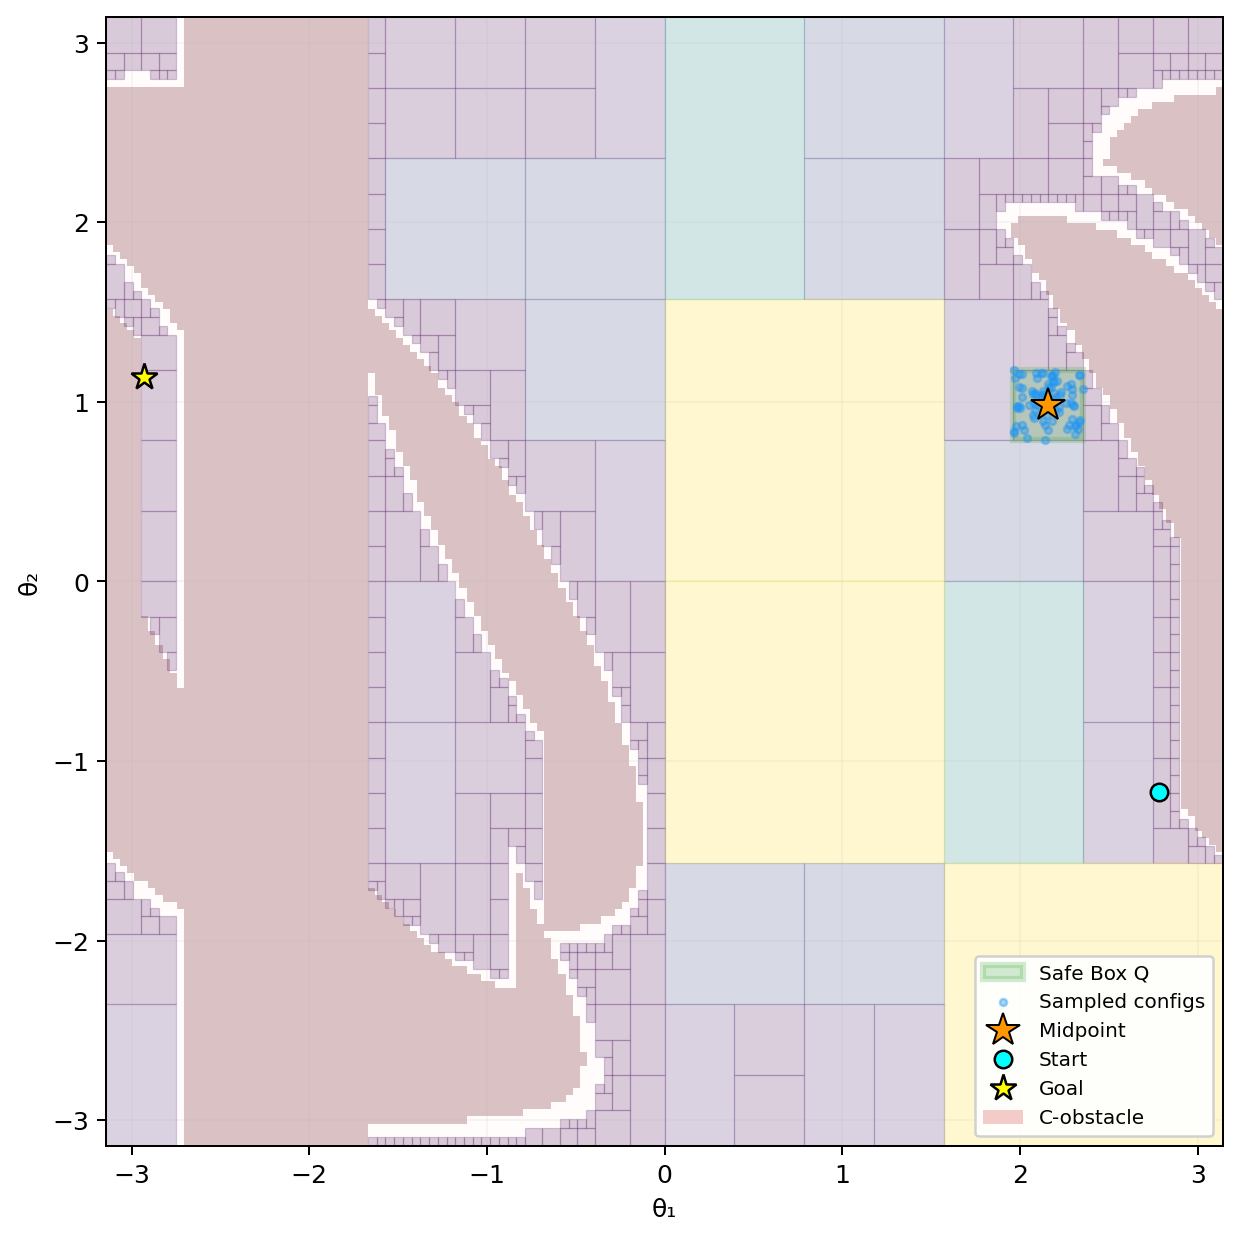
\includegraphics[width=0.292\textwidth]{figures/sbf_grow_1.png} &
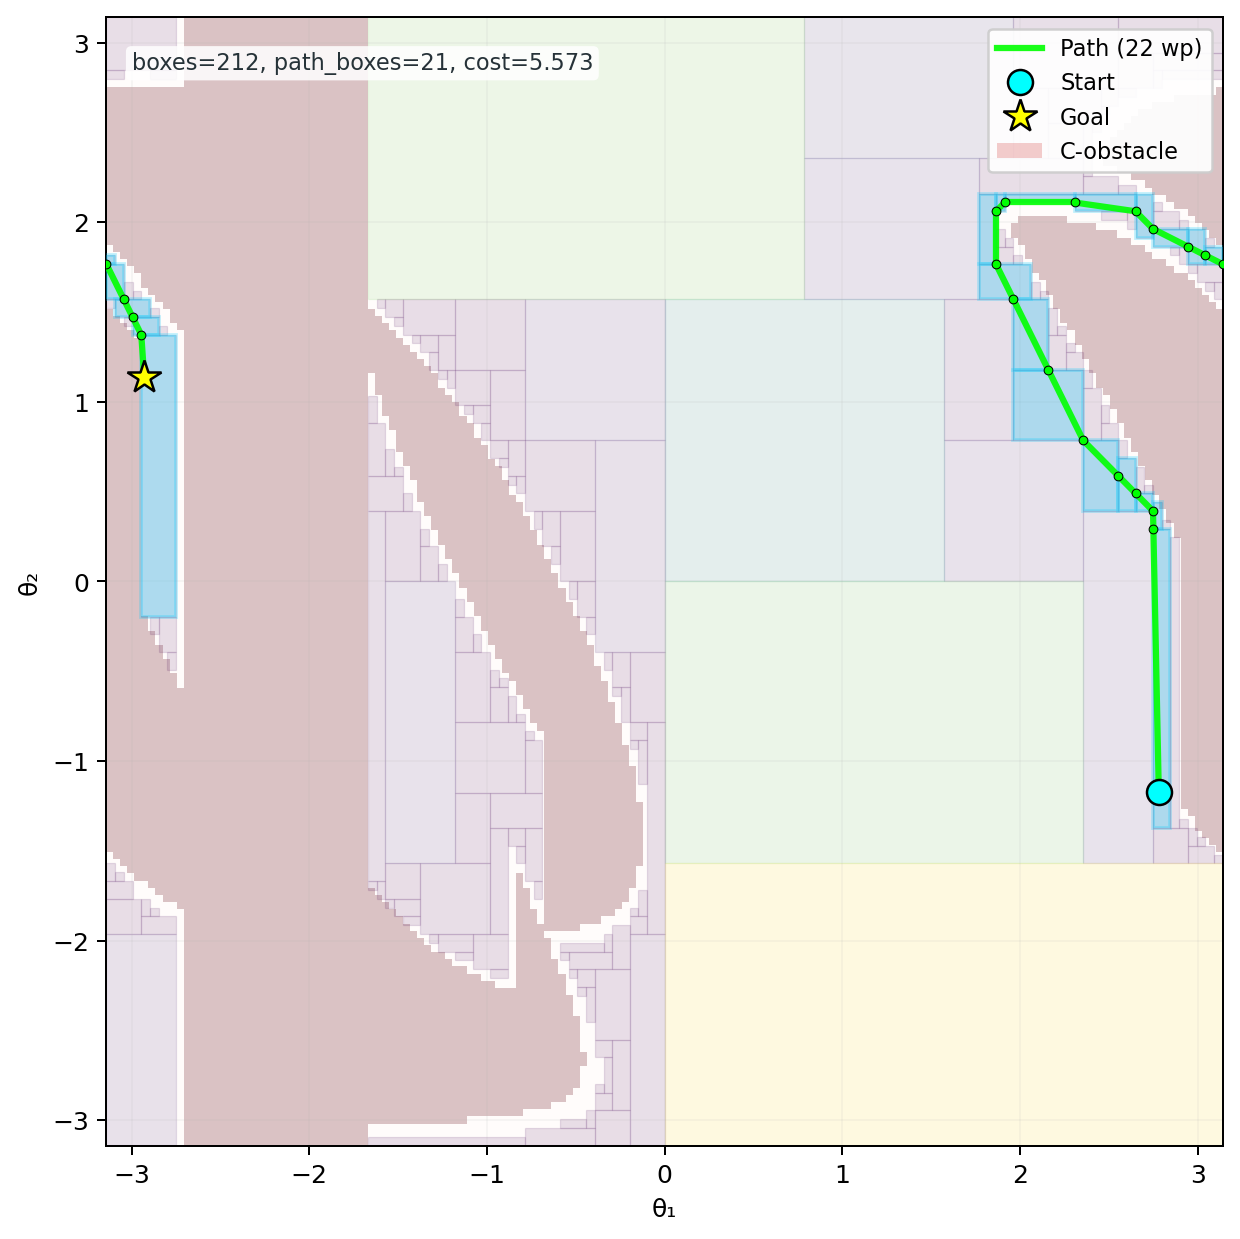
\includegraphics[width=0.292\textwidth]{figures/sbf_grow_3.png} &
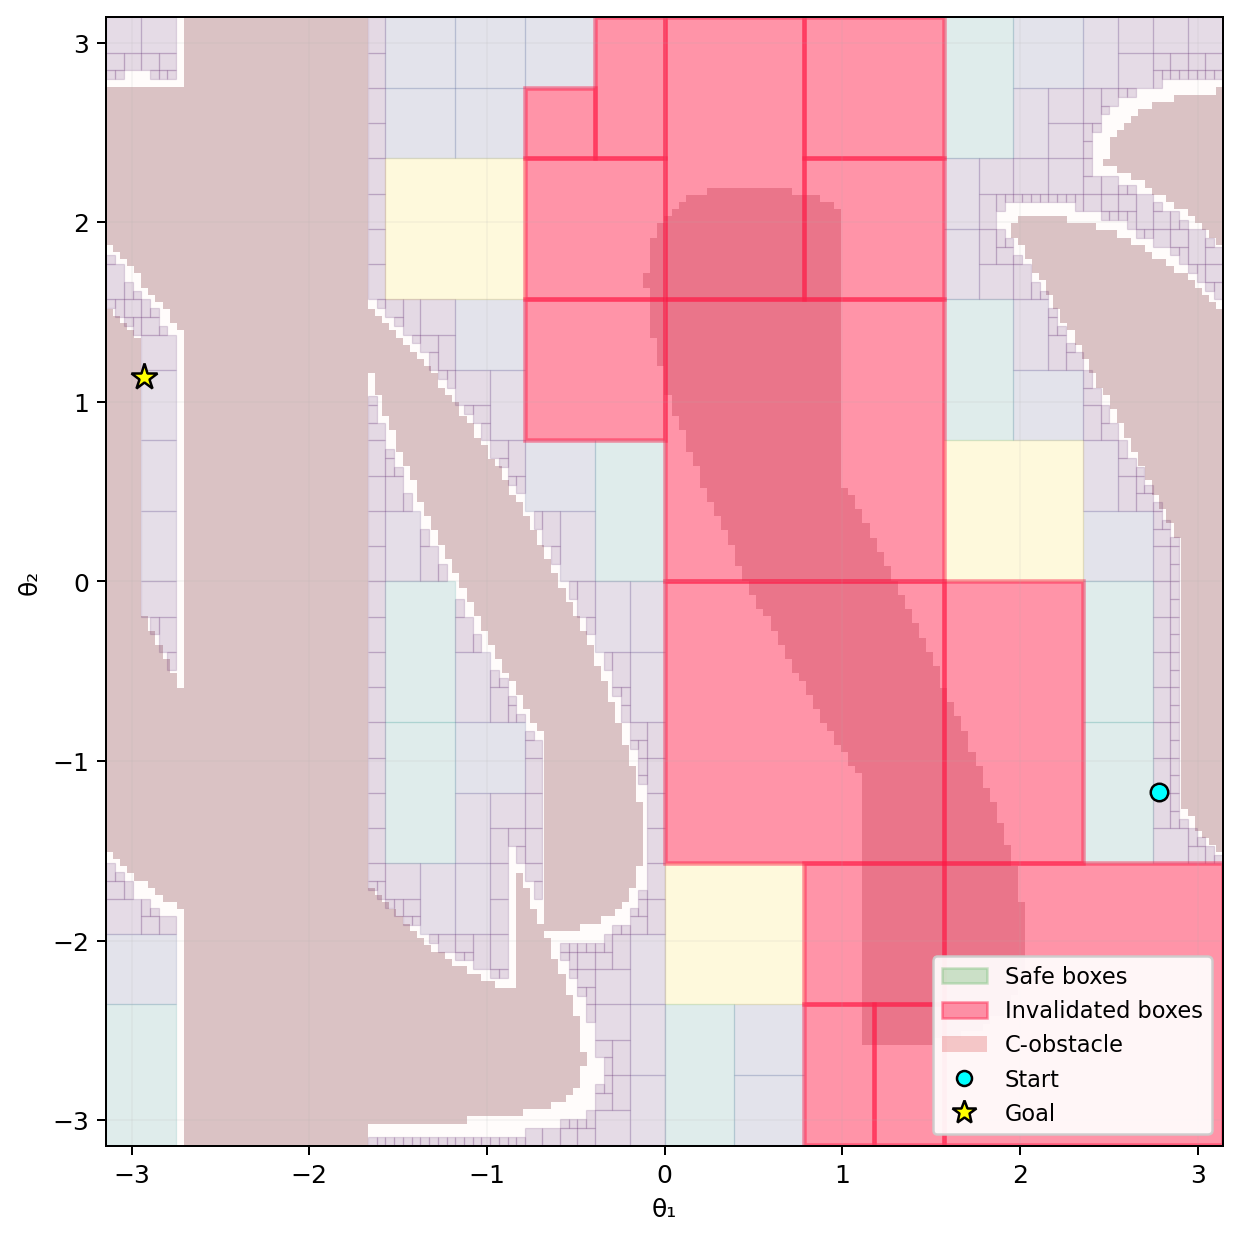
\includegraphics[width=0.292\textwidth]{figures/sbf_grow_5.png} \\
{\footnotesize (a) \cspace{} cells \& selected box} &
{\footnotesize (b) \cspace{} path} &
{\footnotesize (c) Invalidated boxes} \\[2pt]
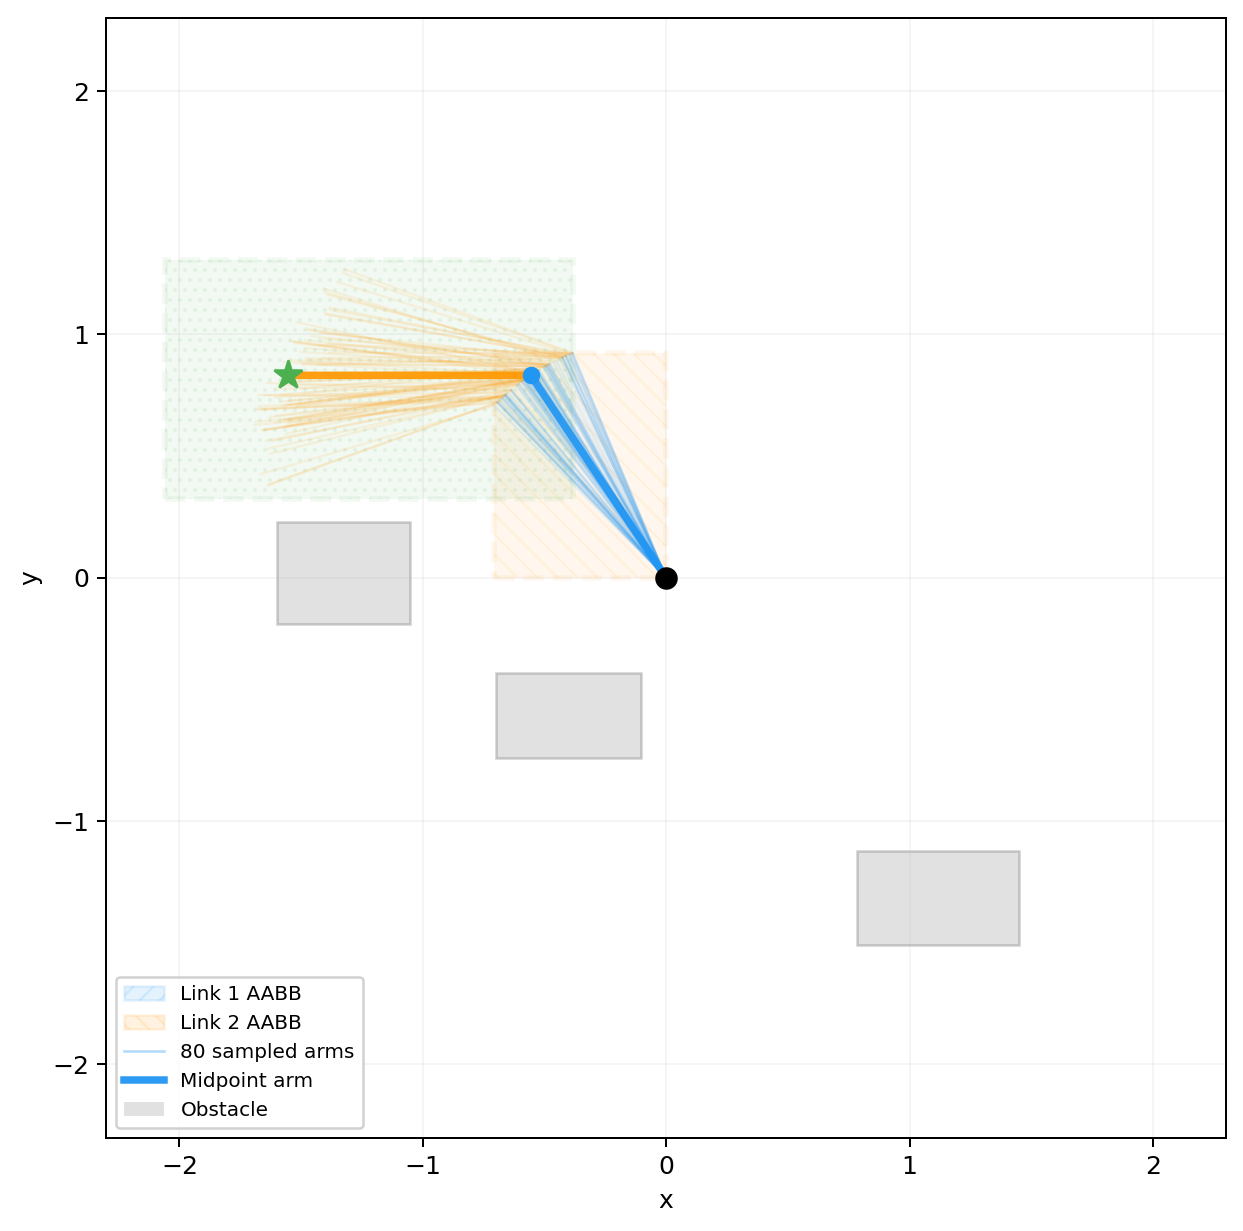
\includegraphics[width=0.292\textwidth]{figures/sbf_grow_2.png} &
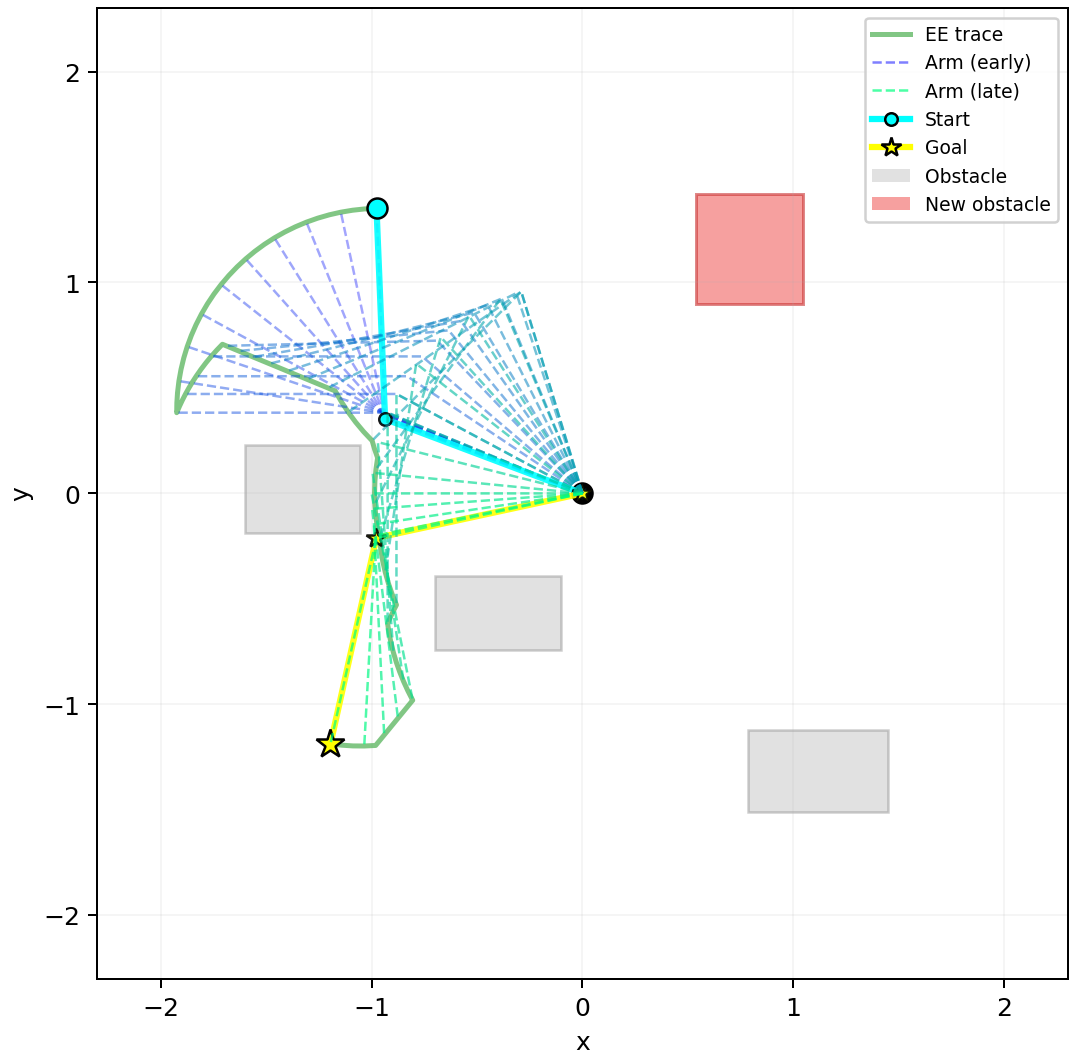
\includegraphics[width=0.292\textwidth]{figures/sbf_grow_4.png} &
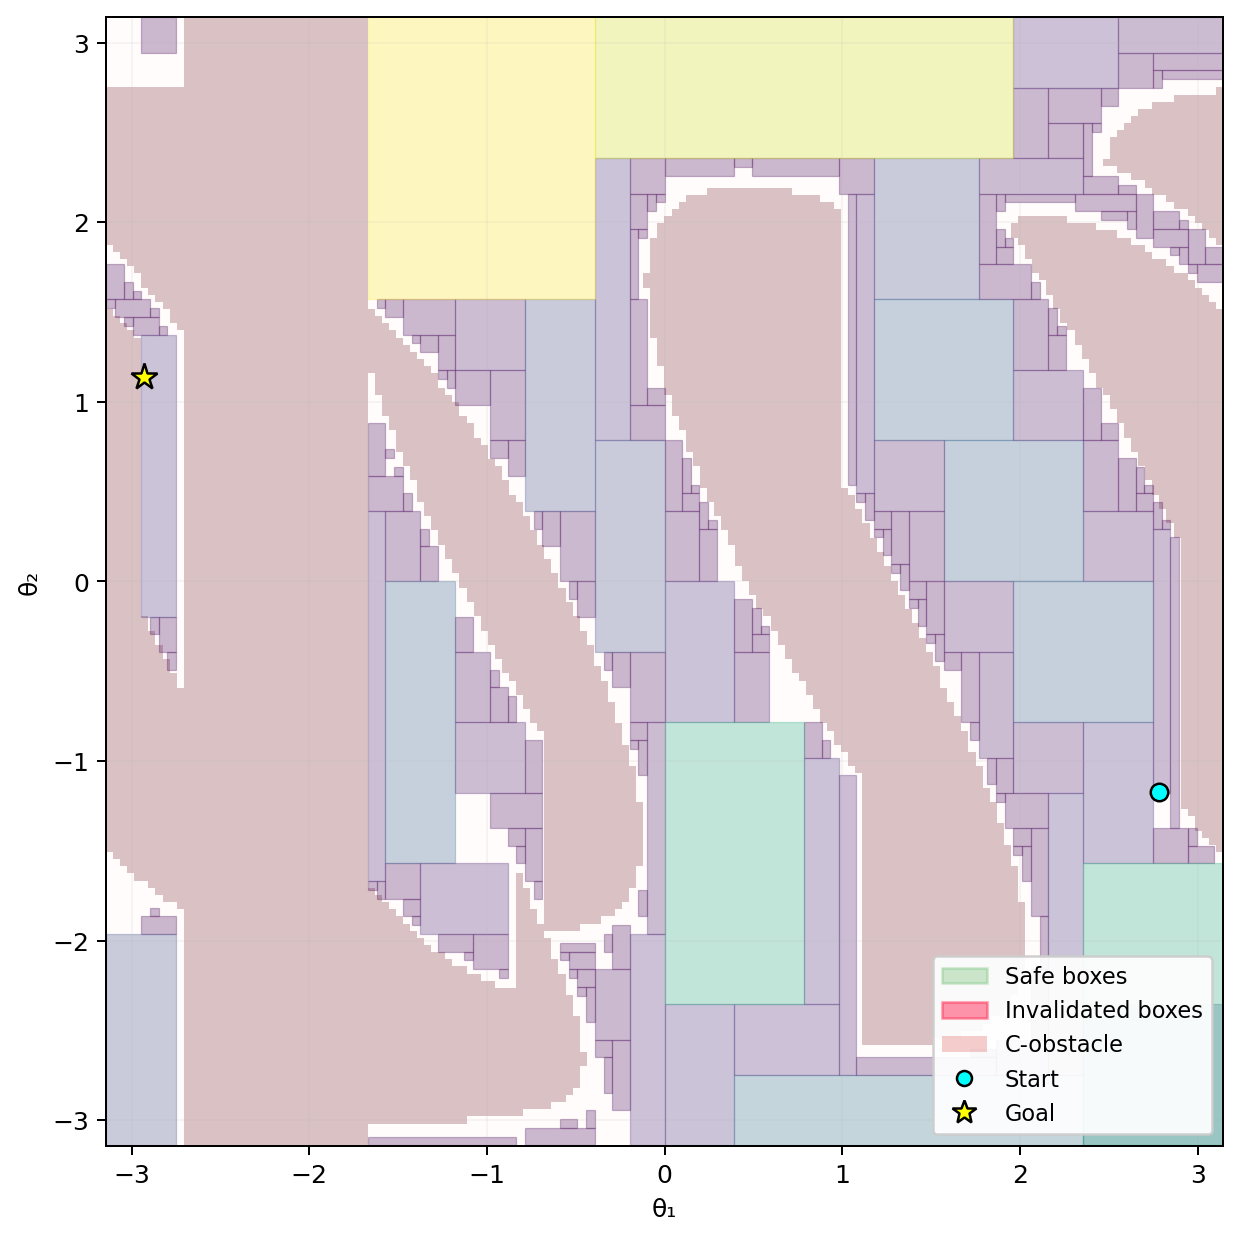
\includegraphics[width=0.292\textwidth]{figures/sbf_grow_6.png} \\
{\footnotesize (d) Workspace AABBs} &
{\footnotesize (e) Workspace path} &
{\footnotesize (f) After regrowth} \\
\end{tabular}
\caption{Two-link schematic of the \rbf{} build, query, and update cycle. A
\cspace{} box maps to workspace axis-aligned bounding boxes (AABBs); a
box-corridor supplies the path; obstacle insertion triggers local refill. Panels
show schematic logic, not experiment geometry; in (e), traces and arm labels
denote schematic poses.}
\label{fig:overview}
\end{figure*}

\section{Lifelong Envelope Cache Tree}\label{sec:lect}

LECT makes warm scene construction inexpensive without turning old obstacle
labels into new certificates. Its invariant is evidence/label separation: it
stores scene-independent endpoint and link-envelope evidence keyed by robot
kinematics and joint intervals, while obstacle tests, box labels, graph
connectivity, and query outcomes remain scene-local. Every replayed envelope is
therefore checked against the current obstacle set.

\subsection{Cache Key and Split Policy}\label{sec:lect_design}

LECT is a dynamically grown binary \(k\)-d tree over $\Q$. A node
stores its joint interval, split metadata, cached endpoint and derived
link-envelope evidence, and runtime residency state. The central invariant is
that evidence is
\emph{kinematics-keyed} rather than \emph{scene-keyed}: replay imports geometry
bounds, not scene-validation labels or graph edges.

\paragraph{Evidence/label separation}
An envelope record is replay-compatible only when the robot model, endpoint
source, envelope representation, split descriptor, link radii, and active-link
set match the current build. The split policy is part of this descriptor, so
alternative policies define distinct cache descriptors. A descriptor match permits
reuse of geometry bounds only; it never imports scene-validity labels. For a
parent interval $I$, let
$I_d^{-}$ and $I_d^{+}$ be the two children
obtained by splitting joint dimension $d$ at its midpoint. Define the cumulative
downstream envelope volume as
\[
\mathcal{V}(I) := \sum_{\ell} \operatorname{vol}(B_\ell(I)).
\]
Here \(\operatorname{vol}(\cdot)\) denotes workspace volume.
One implemented schedule chooses depth-wise split dimensions that minimize the
worst-child cumulative envelope volume,
\[
d^* = \arg\min_d
\max\!\left\{\mathcal{V}(I_d^-),\mathcal{V}(I_d^+)\right\}.
\]
Depth-synchronous schedules keep replay deterministic; if the scheduled
dimension is unavailable at a node, the runtime falls back to the widest valid
dimension. Candidate dimensions are filtered by active-link reachability:
splitting a joint that cannot affect any retained endpoint cannot tighten the
downstream envelopes and is skipped for that descriptor.

\paragraph{Sparse interval staging}
Planning cells need not materialize every ancestor. Each cell stores its exact
joint interval, split counts, and descriptor fingerprint, which identifies the
endpoint source, envelope representation, split policy, link radii, and
active-link set used to interpret replay records. If no exact replay record is
present, the runtime materializes the interval under that descriptor before
validation.

\subsection{Runtime Use and Validation Semantics}

LECT serves local box materialization; graph search uses the scene forest. Given
a joint interval, the runtime replays or materializes endpoint evidence, derives
the requested link representation, and applies the current scene-validation
policy. In the evaluated pipeline, AABB broadphase precedes SupportHull/GJK
refinement. Parent or child records can accelerate materialization, but replayed
evidence alone is not a collision-free certificate. When the required child
records are present, their hulls can tighten an ancestor envelope; the
reconstructed record remains representation-dependent and must still pass the
current scene-validation policy.
Directional records are staged filters: a joint interval first passes the
padded AABB broadphase, and only the remaining close obstacle candidates reach
slab or SupportHull/GJK refinement. If no exact replay record exists, the
interval is materialized on demand and then handled by the same validation path,
so a cache miss changes cost, not semantics or validation responsibility.

\subsection{Storage and Warm-Build Semantics}\label{sec:lect_storage}

Persistence is selective. Endpoint records and derived link-envelope records are
the reusable evidence units. IFK+AABB records can be regenerated on demand.
Non-AABB envelope records are stored only when their additional rejection power
offsets lookup and storage cost. The prewarm pass fills target leaf envelope
records and derives ancestor hulls from child evidence. This
avoids recomputing direct forward kinematics independently at every ancestor
depth. In a warm build, a cache hit reconstructs the requested link envelopes;
the scene builder then checks those envelopes under the current
scene-validation policy. Warm builds still choose and grow scene-specific boxes;
no persisted box label is imported as a certificate. The Shelf replay used in
the experiments is read-only during timing, so the replay store does not
accumulate new evidence during those measurements. Random-scene cache growth is
treated separately as part of the per-robot profile.

% ==============================================================================
\section{RapidBoxForest Construction}\label{sec:forest}

This section turns envelope validation and LECT replay into a query-agnostic
scene structure. Fig.~\ref{fig:overview} illustrates the planning layer:
\rbf{} builds scene-specific policy-accepted \cspace{} boxes and stores their
adjacency in a typed corridor graph. For a fixed obstacle set, later queries use
box membership and graph search instead of rebuilding the cover. LECT remains a
separate evidence store, and each scene box is checked against the current
obstacles.

\begin{algorithm}[t]
\caption{Local box materialization around a seed.}
\label{alg:ffb_rewrite}
\footnotesize
\begin{algorithmic}[1]
\REQUIRE Seed $q$, LECT tree $\mathcal{T}_L$, obstacle set $\calO$, validation
policy $V_{\calO}$, descriptor $\delta$, depth cap $D_{\max}$
\ENSURE Accepted interval with status, or failure with retained domain
\STATE $I\leftarrow$ root interval of $\mathcal{T}_L$ that contains $q$; $d\leftarrow0$
\WHILE{$d\le D_{\max}$}
  \STATE $R\leftarrow\operatorname{ReplayOrMaterialize}(\mathcal{T}_L,I,\delta)$
  \STATE derive active-link envelopes $\{B_\ell(I)\}$ from endpoint record $R$
  \STATE $s\leftarrow V_{\calO}(\{B_\ell(I)\},\calO)$
  \STATE \textit{$s$ is free, blocked, or inconclusive under the active policy}
  \IF{$s$ is free under a conservative policy}
    \RETURN $(I,\mathrm{certificate}\mbox{-}\mathrm{backed})$
  \ELSIF{$s$ is free only under a filter policy}
    \RETURN $(I,\mathrm{validation}\mbox{-}\mathrm{required})$
  \ENDIF
  \IF{$d=D_{\max}$}
    \RETURN failure with retained domain $(I,s)$
  \ENDIF
  \STATE choose split dimension from $\delta$; fall back to widest active dimension
  \STATE $I\leftarrow$ child of $I$ that contains $q$; $d\leftarrow d+1$
\ENDWHILE
\RETURN failure
\end{algorithmic}
\end{algorithm}

A box is an axis-aligned joint interval
$B=[l^{(1)},u^{(1)}]\times\cdots\times[l^{(n)},u^{(n)}]\subseteq\Q$.
A \emph{policy-accepted box} has passed the configured scene-validation policy.
Conservative link-envelope disjointness makes acceptance a collision-free
certificate; a non-conservative filter makes the box only a planning region, so
any path segment using it remains validation-required. Rejected cells are
excluded from the forest, while selected blocked or inconclusive domains are
retained for local refinement or later update.

\subsection{Construction Objective}\label{sec:forest_objective}

The construction objective is a budgeted reusable cover, not an exhaustive
decomposition of \(\Cfree\). Given the joint-limit box $\Q$ and obstacle set
$\calO$, let \(V_{\calO}(B)\) denote the configured scene-validation predicate
for a box \(B\). The build stage constructs a forest \(\mathcal{F}\)
of \(N\) retained boxes satisfying
\[
\begin{gathered}
\mathcal{F}=\{B_1,\ldots,B_N\},\\
B_i\subseteq\Q,\quad V_{\calO}(B_i),\quad i=1,\ldots,N.
\end{gathered}
\]
The reusable output is $(\mathcal{F},G)$, where \(G\) is the typed corridor
graph storing adjacency and auxiliary transitions; the box budget targets
anchors, frontiers, and connectors.

For two boxes
\[
B_i=\prod_{d=1}^{n}[l_i^{(d)},u_i^{(d)}],\qquad
B_j=\prod_{d=1}^{n}[l_j^{(d)},u_j^{(d)}],
\]
let \(\varepsilon_c\ge 0\) denote the connection tolerance. \rbf{} treats the
boxes as connected when the closed intervals in every coordinate overlap or have
a gap no larger than \(\varepsilon_c\):
\[
\max\{l_i^{(d)},l_j^{(d)}\}
\le
\min\{u_i^{(d)},u_j^{(d)}\}+\varepsilon_c,\qquad d=1,\ldots,n.
\]
Only exact overlap or contact directly yields a contained box-corridor.
Tolerance-gap and explicit segment edges are graph-search aids, not
certificates, unless they are converted into conservative box-corridor or
finite-cover OBB-corridor regions; otherwise they require fixed-step validation.

\subsection{Build Pipeline}

The build proceeds through four stages. First, local materialization descends
the LECT tree around a seed and returns the first interval accepted by the
configured scene policy. Second, a priority leaf sweep classifies cells near
anchors, frontiers, and uncovered query-relevant domains. Third, restricted
refinement revisits retained blocked or inconclusive domains under a separate
budget. Finally, consolidation merges or removes boxes only after revalidating
the resulting box. \Cref{alg:ffb_rewrite,alg:leaf_sweep_refine} make these
decisions explicit; all stages use the same materialize--validate--connect
pattern, so later graph search never relies on an unvalidated scene label.

\paragraph{Controls}
Validation semantics and timings are governed by the build budget, LECT
descriptor, endpoint and link representation, admitted edge types, and
validation resolution. The fixed profile uses saved anchors, query endpoints,
frontier domains, and repair witnesses as seeds; priority favors anchor and
connector coverage before uncovered frontier volume, with deterministic
tie-breaking. Splits follow the LECT descriptor schedule, profile budgets are
fixed before evaluation, and candidate merges are kept only after revalidation.
Materialization failures remain deferred domains for restricted refinement;
frontier and repair witnesses follow the status rules in
\Cref{tab:claim_boundary}. In Algorithms~\ref{alg:ffb_rewrite} and~\ref{alg:leaf_sweep_refine},
\(\mathcal{T}_L\), \(D_{\max}\), and \(\mathcal{C}\) denote the LECT tree, the
descent depth cap, and the retained blocked or inconclusive collision-domain
cache.

\begin{algorithm}[!t]
\caption{Adaptive leaf sweep and local refinement.}
\label{alg:leaf_sweep_refine}
\footnotesize
\begin{algorithmic}[1]
\REQUIRE Seed/anchor set $\mathcal{S}$, LECT tree $\mathcal{T}_L$, obstacle set
$\calO$, validation policy $V_{\calO}$, sweep and refinement budgets
\ENSURE Scene forest $\mathcal{F}$, typed graph $G$, retained domains $\mathcal{C}$
\STATE initialize priority queue $\mathcal{P}$ using the fixed priority policy
\STATE $\mathcal{F}\leftarrow\emptyset$; $G\leftarrow\emptyset$; $\mathcal{C}\leftarrow\emptyset$
\WHILE{$\mathcal{P}$ is nonempty and sweep budget remains}
  \STATE pop the highest-priority cell or seed domain from $\mathcal{P}$
  \STATE call Algorithm~\ref{alg:ffb_rewrite}; if the domain is fixed, materialize that exact cell
  \IF{an accepted box $B$ is returned}
    \STATE insert $B$ into $\mathcal{F}$ and connect overlap/contact neighbors in $G$
    \STATE propose connector, gap, segment, OBB, and repair transitions within the fixed profile budget
    \STATE convert eligible transitions to conservative corridors; insert each edge in $G$ with the status in \Cref{tab:claim_boundary}
    \STATE enqueue adjacent frontier domains not already covered by $\mathcal{F}$
  \ELSE
    \STATE retain the blocked or inconclusive domain in $\mathcal{C}$
    \STATE split by the descriptor policy and re-enqueue children while the refinement budget allows
  \ENDIF
\ENDWHILE
\FORALL{retained domains selected from $\mathcal{C}$}
  \STATE refine locally; insert only boxes that pass $V_{\calO}$ and remain in the domain
\ENDFOR
\FORALL{candidate merges or redundant boxes}
  \STATE replace boxes only if the merged or retained box passes the same validation rule
\ENDFOR
\RETURN $\mathcal{F},G,\mathcal{C}$
\end{algorithmic}
\end{algorithm}

Exact-cell materialization means replaying or computing evidence for the retained
cell itself rather than descending from a seed-containing ancestor. This keeps
edit, refill, and repair domains aligned with the scene-cache labels that caused
the revisit.

\FloatBarrier
\subsection{Corridor Query and Certificate}
\label{sec:forest_graph}

\begin{samepage}
The graph is typed because search connectivity and certificate-carrying
connectivity need not coincide. After consolidation, $G$ has policy-accepted
vertices and edge types
$E_{\cap}$ (overlap/contact), $E_{\varepsilon}$ (tolerance gap), $E_s$
(segment), $E_o$ (finite-cover OBB-corridor), and $E_{\pi}$ (repair witness).
As summarized in \Cref{tab:claim_boundary}, overlap/contact edges and
finite-cover OBB-corridor edges carry certificates only when backed by
conservative region checks. Repair-witness edges carry certificates only after
conversion into a conservative box-corridor or OBB-corridor representation.
Certificate status is determined by the backing conservative region check, not
by the edge label alone.
\end{samepage}

\begin{samepage}
Given start and goal configurations, the query locates containing boxes or
configured anchor boxes and searches $G$. The certificate applies only to
returned paths contained in conservative box regions or finite-cover
OBB-corridor regions. \Cref{lem:corridor_certificate} states the box-region
case; \Cref{sec:obb_endpoint_env} gives the finite-cover certificate for
OBB-corridor edges. All other returns follow the validation-required semantics in
\Cref{tab:claim_boundary}.
\end{samepage}

\begin{samepage}
\begin{lemma}[Box-corridor certificate]
\label{lem:corridor_certificate}
Let $\mathcal{F}$ be a forest whose boxes have each passed conservative
link-envelope validation against obstacle set $\calO$. Let
\(R_{\mathcal{F}}:=\bigcup_{B\in\mathcal{F}}B\) denote the represented box
union. If a continuous path $\gamma:[0,1]\to\Q$ satisfies
\(\gamma([0,1])\subseteq R_{\mathcal{F}}\), then every configuration on
$\gamma$ is collision-free with respect to the collision model in
\Cref{ass:collision_model}.
\end{lemma}
\end{samepage}

\begin{proof}
For any $s\in[0,1]$, containment gives a conservatively validated box
$B\in\mathcal{F}$ with $\gamma(s)\in B$. By conservative link-envelope
validation and \Cref{cor:box_validation}, the robot geometry at $\gamma(s)$ is
disjoint from $\calO$. Since $s$ was arbitrary, the whole path is
collision-free.
\end{proof}

\noindent\emph{Certificate interpretation.}
The lemma certifies collision-freedom for paths contained in conservatively
validated regions. It does not imply coverage or completeness: finite depth,
axis-aligned boxes, envelope overapproximation, and bridge or repair limits can
miss paths. Returns that leave certified regions, include residual non-corridor
segments, are post-processed, or traverse boxes admitted by non-conservative
filters follow the validation-required semantics in \Cref{tab:claim_boundary}.

\begin{figure}[!t]
  \centering
  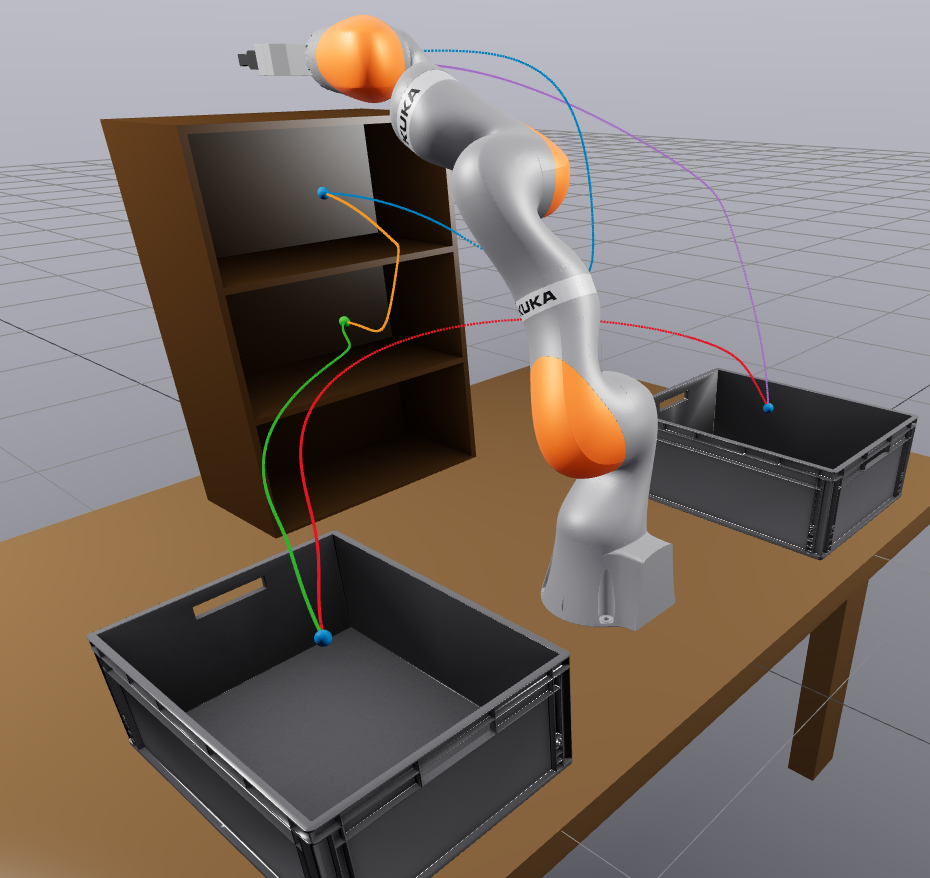
\includegraphics[width=0.94\columnwidth]{figures/Marcucci_scene.png}
  \caption{Canonical Marcucci Shelf+KUKA LBR iiwa (Shelf+IIWA) scene with
  saved anchors: approach-side (AS), target-shelf (TS), center-shelf (CS),
  left-bin (LB), and right-bin (RB).}
  \label{fig:tro_shelf_scene}
\end{figure}

\section{Experiments}\label{sec:exp}

The evaluation is organized as an evidence chain. Q1 tests the intended warm
reuse mechanism on the Shelf+KUKA LBR iiwa (Shelf+IIWA) scene. Q2 places that
fixed profile against roadmap, sampling, and convex-region baselines. Q3 checks
whether the same reusable-forest behavior holds across saved random scenes and
three robot models. Q4 explains the mechanism choices behind the default
profile, and Q5 isolates local edit maintenance.

\begin{table*}[!t]
\centering
\caption{Evaluation map. Each question is tied to one writing claim and one
accounting boundary so the experimental narrative stays aligned with
\Cref{tab:claim_boundary}.}
\label{tab:evaluation_map}
\footnotesize
\setlength{\tabcolsep}{2.6pt}
\renewcommand{\arraystretch}{1.00}
\begin{tabular}{@{}M{0.08\textwidth}M{0.25\textwidth}M{0.28\textwidth}M{0.30\textwidth}@{}}
\toprule
Question & Writing claim & Main evidence & Boundary emphasized \\
\midrule
Q1 Shelf replay & LECT replay lowers reusable scene-build cost. & Fixed b100 Shelf profile, d23 cache, five-anchor cycle. & Replay imports geometry evidence only; success requires the same final validation. \\
Q2 Shelf context & \rbf{} occupies a low-build middle point. & PRM, RRT-Connect, BIT*, and IRIS/GCS on the same saved cycle. & Build/5 + \onlineq{} is the reuse-horizon display, not an optimality claim. \\
Q3 Random scenes & Reusable forests generalize across robots and scene difficulty. & Three-robot medium/hard catalogs. & \rbf{} is not claimed as fastest single-query planning. \\
Q4 Mechanisms & Endpoint and link-envelope choices explain the default profile. & Endpoint-source and narrow-phase mechanism tables. & Mechanism rows are not end-to-end planning rows. \\
Q5 Edits & Local scene-cache maintenance is isolated from warm rebuild cost. & Obstacle insertion/removal maintenance timing. & Maintenance-only timing excludes post-edit query success. \\
\bottomrule
\end{tabular}
\end{table*}

\paragraph{Protocol}
Timings were measured on Ubuntu 22.04 with an Intel i5-12600KF central
processing unit (CPU) and 31~gibibytes (GiB) of random-access memory (RAM). All
\rbf{}, LECT, and OMPL comparison rows use the common 8-thread wall-clock
policy. The generated tables and figures store data sources, simplification
settings, checksums, and integrity metadata.

For planning tables, Build is reusable scene-construction time before the timed
queries. \onlineq{} is planner online time after a reusable build; it excludes
final simplification and the post-run validation pass. Success nevertheless
requires fixed-step validation with a 0.01~rad segment step unless a row is
explicitly marked conservative. Thus claims using \onlineq{} are planner-time
claims, not total accepted-path latency; the validation pass is a common
acceptance audit rather than an input to the timing ranks. If a row or
supplementary artifact reports validation or simplification costs, those fields
must be added explicitly before making a total-latency claim; otherwise compact
main-table timings should be read strictly as planner-time comparisons.
Entries report median $[Q_1,Q_3]$ unless the caption states otherwise.
Amortized quantities of the form Build/$K$ + \onlineq{} use $K$ as a stated
reuse horizon, not a success count. Path-length ratios divide the
validated returned path by the same-query empirical reference length;
$L_{\mathrm{ref}}$ denotes that empirical reference, not an optimality
certificate.

Planning rows use the collision model in \Cref{ass:collision_model}: active
rounded links are checked against $\calO$. Self-collision, attachments,
grippers, and task-specific forbidden regions require additional policy checks
before a certificate is claimed.

\paragraph{Cache and profile accounting}
Warm-cache rows include compatible LECT lookup and evidence reads, but exclude
snapshot creation/loading, resident memory, and offline setup amortization. The
\mbox{d23} label identifies a depth-23 LECT cache: 16,777,215 records,
12.75~GiB on disk, and 958.079~s prewarm time. Bridge and repair witnesses
follow \Cref{tab:claim_boundary}: after conservative box-corridor or finite-cover
OBB-corridor conversion they are certificate-backed; otherwise they remain
validation-required transitions. All profile budgets are fixed before producing
the Shelf and random-scene summaries; the b100 Shelf
profile and random-scene OBB-corridor profiles use these fixed budgets unchanged
across saved seeds and robot/difficulty rows, and no row is tuned after observing
validation outcomes.

\begin{table*}[!t]
  \centering
  \begin{minipage}{0.74\textwidth}
  % Auto-generated from current trade-off artifacts.
\begingroup
\centering
\captionof{table}{Shelf+IIWA \rbf{} profile and mechanism ablations.}
\label{tab:tro-shelf-ablation}
\scriptsize
\setlength{\tabcolsep}{2.2pt}
\renewcommand{\arraystretch}{1.02}
\begin{tabular}{@{}lcccc@{}}
\toprule
Case & Build & \onlineq{} & Amort.\ 5q & $L/L^\star$ \\
\midrule
\rbf{} baseline & 0.171 [0.166, 0.174] & 0.077 [0.072, 0.085] & 0.111 [0.107, 0.117] & 1.15 [1.08, 1.39] \\
Critical sample & 0.279 [0.275, 0.283] & 0.087 [0.078, 0.095] & 0.145 [0.134, 0.151] & 1.14 [1.09, 1.38] \\
Link AABB & 0.167 [0.164, 0.171] & 0.083 [0.077, 0.086] & 0.116 [0.111, 0.119] & 1.19 [1.08, 1.48] \\
Live HIFK-5 & 2.770 [2.644, 3.003] & 0.181 [0.139, 0.207] & 0.739 [0.703, 0.777] & 1.15 [1.08, 1.43] \\
SupportHull only & 0.193 [0.188, 0.200] & 0.087 [0.082, 0.095] & 0.126 [0.120, 0.136] & 1.15 [1.08, 1.39] \\
\bottomrule
\end{tabular}
\par\vspace{0.1ex}
{\scriptsize\emph{Notes:} Median \([Q_1,Q_3]\), s. Build is reusable; Amort.\ 5q \(=\) Build/5+\onlineq{}; \onlineq{} excludes simplification/validation. AABB = axis-aligned bounding box; HIFK = hierarchical interval forward kinematics; SupportHull = support-function hull. Critical sample is non-certifying; \(L/L^\star\) uses the same-query 0.01~rad reference.\par}
\par\endgroup

  \end{minipage}
\end{table*}

\begin{figure*}[!t]
  \centering
  {\footnotesize Labels: IRIS/GCS = Iterative Regional Inflation + Graphs of
  Convex Sets; RBF b100 = fixed 100-box Shelf point; Amort.\ 5q =
  Build/5 + \onlineq{}.\par}
  \begin{minipage}[t]{0.34\textwidth}
    \centering
    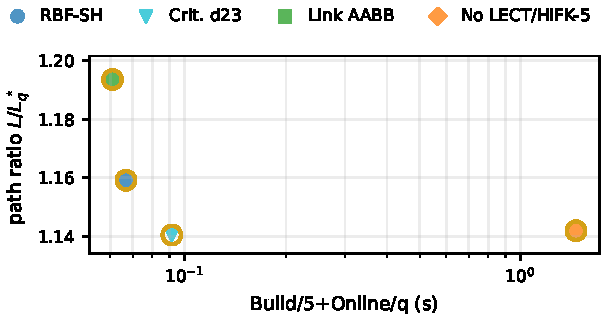
\includegraphics[width=0.96\linewidth,keepaspectratio]{generated/fig_tro_shelf_tradeoff.pdf}
    \caption{Shelf+IIWA mechanism trade-off. Points plot Table~\ref{tab:tro-shelf-ablation}
    Amort.\ 5q versus \(L/\Lref{}\); smaller ratios are shorter, and gold rings
    mark Table~\ref{tab:tro-shelf-ablation} rows.}
    \label{fig:tro_shelf_tradeoff}
  \end{minipage}\hfill
  \begin{minipage}[t]{0.62\textwidth}
    \centering
    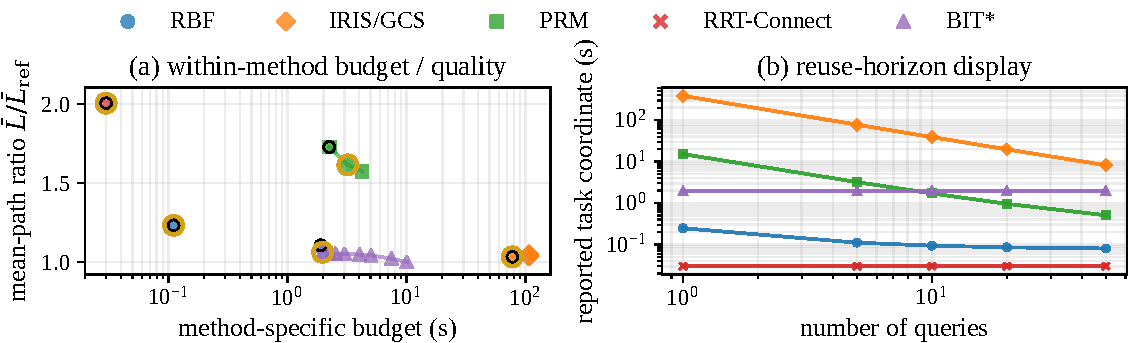
\includegraphics[width=0.96\linewidth,keepaspectratio]{generated/fig_tro_shelf_cross_tradeoff.pdf}
    \caption{Shelf+IIWA cross-algorithm trade-off. Black rings mark first
    successful checkpoints. All rows follow the common 8-thread execution
    policy. The horizontal coordinate is Build/5 + \onlineq{} for reusable
    methods and \onlineq{} for per-query rows with no reusable build; smaller
    \(L/\Lref{}\) is shorter. Right: amortized time per query versus reuse count.}
    \label{fig:tro_shelf_cross_tradeoff}
  \end{minipage}
\end{figure*}

\begin{table*}[!t]
  \centering
  \TableFontRestore
  % Auto-generated from current trade-off artifacts.
\begingroup
\centering
\captionof{table}{Common-rule tabulated Shelf+IIWA rows from Fig.~\ref{fig:tro_shelf_cross_tradeoff}, reported by query. Gold rings in the figure mark these rows only to expose detailed numeric values; the full curves remain the primary evidence. RBF uses the current leaf-sweep--RRT grower profile. PRM, RRTConnect, and BIT* are current reruns with old TRO baseline budgets; the IRIS-NP+GCS per-query entries are the audited old TRO artifact. OMPL planning, final simplify, and fixed-resolution final audit use the same 0.01 joint-space segment step.}
\label{tab:tro-shelf-cross-algorithm}
\footnotesize
\setlength{\tabcolsep}{1.55pt}
\renewcommand{\arraystretch}{0.96}
\begin{tabular}{@{}lrr|rr|rr|rr|rr@{}}
\toprule
  & \multicolumn{2}{c}{\textbf{\footnotesize \shortstack{RBF b100\\[-0.2ex]{\normalfont\fontsize{7.1}{7.8}\selectfont Build 0.356\,s; SR 8/8}}}} & \multicolumn{2}{c}{\textbf{\footnotesize \shortstack{IRIS-NP+GCS\\[-0.2ex]{\normalfont\fontsize{7.1}{7.8}\selectfont Build 753.000\,s; SR 1/1}}}} & \multicolumn{2}{c}{\textbf{\footnotesize \shortstack{PRM\\[-0.2ex]{\normalfont\fontsize{7.1}{7.8}\selectfont Build 6.764\,s; SR 8/8}}}} & \multicolumn{2}{c}{\textbf{\footnotesize \shortstack{RRTConnect\\[-0.2ex]{\normalfont\fontsize{7.1}{7.8}\selectfont Build 0.006\,s; SR 8/8}}}} & \multicolumn{2}{c}{\textbf{\footnotesize \shortstack{BIT*\\[-0.2ex]{\normalfont\fontsize{7.1}{7.8}\selectfont Build 0.007\,s; SR 8/8}}}} \\
\cmidrule(lr){2-3}\cmidrule(lr){4-5}\cmidrule(lr){6-7}\cmidrule(lr){8-9}\cmidrule(lr){10-11}
Query & Query (s) & Path & Query (s) & Path & Query (s) & Path & Query (s) & Path & Query (s) & Path \\
\midrule
AS$\rightarrow$TS & 0.074 & 2.43 & 0.558 & 2.38 & 0.409 & 3.22 & 0.001 & 2.30 & 0.001 & 4.59 \\
TS$\rightarrow$CS & 0.004 & 1.10 & 0.463 & 1.99 & 0.410 & 0.69 & 0.001 & 1.18 & 0.001 & 0.69 \\
CS$\rightarrow$LB & 0.004 & 2.27 & 0.533 & 2.63 & 0.411 & 2.02 & 0.001 & 2.74 & 0.001 & 4.82 \\
LB$\rightarrow$RB & 0.042 & 3.09 & 0.825 & 3.26 & 0.345 & 4.32 & 0.001 & 2.55 & 0.001 & 6.03 \\
RB$\rightarrow$AS & 0.028 & 3.69 & 0.765 & 1.84 & 0.407 & 4.80 & 0.001 & 4.59 & 0.001 & 5.33 \\
\bottomrule
\end{tabular}
\par\endgroup

\end{table*}

\subsection{Q1: Shelf+IIWA Replay and Fixed Profile}
\label{sec:exp_shelf_iiwa}

Q1 tests whether LECT replay lowers reusable build cost without changing path-acceptance responsibility. Fig.~\ref{fig:tro_shelf_scene}
shows the Shelf+IIWA scene and fixed five-anchor query cycle with approach-side
(AS), target-shelf (TS), center-shelf (CS), left-bin (LB), and right-bin (RB)
anchors; the executed order is AS--TS--CS--LB--RB--AS\@. Table~\ref{tab:tro-shelf-ablation}
and Fig.~\ref{fig:tro_shelf_tradeoff} report the fixed 100-box Shelf profile
(b100) over seeds 0--7. The cycle is used for mechanism ablations and profile
selection; saved random-scene catalogs below test broader start-goal variation.

The b100 \rbf{} baseline uses SupportHull link envelopes replayed from the d23
cache: Build 0.171~s, \onlineq{} 0.077~s, and five-query amortized time 0.111~s;
Table~\ref{tab:tro-shelf-ablation} gives quartiles. The \mbox{Live HIFK-5} row
keeps the same depth and validation budget but computes evidence live, giving a
2.770~s reusable build; the other rows replay d23 evidence.
After OBB-corridor conversion, the 40 validated Shelf paths in
Table~\ref{tab:tro-shelf-ablation} contain no residual non-corridor segments.
The representation rows isolate implementation choices: Link~AABB changes \onlineq{} from
0.077~s to 0.083~s while changing the median \(L/\Lref{}\) from 1.15 to 1.19;
\mbox{SupportHull-only} raises the five-query amortized time from 0.111~s to
0.126~s.

The Shelf profile table follows the guarantee matrix: converted corridor
segments carry certificates, and any remaining acceptance is audited by the fixed
0.01~rad validation step. In the reported fixed pipeline, all 40 paths pass that
audit. A disabled-pipeline ablation with the query bridge, repair, shortcutting,
and final simplification all turned off is included only as a full-pipeline
consistency check; it should not be read as a single-stage failure diagnosis.

\noindent\emph{Takeaway.}
LECT replay reduces the reusable build by about 16.2$\times$ relative to live
\mbox{HIFK-5} under the same fixed profile, while success remains anchored in
the same path-acceptance rules in \Cref{tab:claim_boundary}.

\subsection{Q2: Shelf Cross-Algorithm Context}
\label{sec:exp_shelf_cross_algorithm}

Q2 tests the cross-algorithm context of the fixed \rbf{} profile. The study
applies the same five queries, 0.01~rad validation segment step, 0.010~s
final-simplification budget, and 8-thread execution policy to \rbf{},
\mbox{IRIS/GCS}, PRM, \mbox{RRT-Connect}, and BIT*. \rbf{} uses the b100
profile and per-query \onlineq{}; PRM and \mbox{IRIS/GCS} report reusable
builds, while \mbox{RRT-Connect} and BIT* remain per-query rows with no reusable
build term under the same thread budget. BIT* checkpoints are offline
quality--time references, not online stopping rules.

Under these definitions, reusable builds are 0.171~s (\rbf{}), 20.040~s
(PRM), and 355.425~s (\mbox{IRIS/GCS}). The \rbf{} build excludes d23
prewarm, snapshot loading costs, and resident memory. In the per-query \(T\)
columns, \mbox{RRT-Connect} has lower \(T\) than \rbf{} in all five Shelf
queries but has higher \(L/\Lref{}\) in all five; BIT* has higher \(T\) than
\rbf{} but lower \(L/\Lref{}\) in all five. This timing--quality comparison is
limited to the saved five-query cycle and its stated reusable build accounting.

\noindent\emph{Takeaway.}
On this fixed cycle, \rbf{} is the low-build middle point: it avoids the large
reusable builds of PRM and \mbox{IRIS/GCS} while returning shorter validated
paths than \mbox{RRT-Connect}. The same data should not be read as a shortest-path
or fastest-single-query claim, because BIT* is shorter and \mbox{RRT-Connect} is
faster per query in this saved cycle.

\FloatBarrier
\subsection{Q3: Random Multi-Robot Scenes}
\label{sec:exp_generalization}

Q3 tests whether reusable box forests remain useful beyond the Shelf profile.

\begin{table*}[!t]
  \centering
  \TableFontRestore
  \begin{table*}[t]
\centering
\caption{Saved-catalog random-scene reusable-planner best trade-off points. Each obstacle scene stores fixed multi-query batches; RBF builds once per scene and online timings reuse the offline forest. Online/q excludes final simplification; Simplify/q reports the measured cost under the globally fixed 0.01~s OMPL post-processing budget. Times exclude final audit; full box-budget and amortization curves are shown in Fig.~\ref{fig:tro_random_tradeoff}.}
\label{tab:tro-random-summary}
\footnotesize
\begin{tabular}{llrrrrrrrrr}
\toprule
Robot & Difficulty & Boxes & SR & Build & Online/q & Simplify/q & Amort@10 & Path & Seg. \\
\midrule
iiwa & easy & 800 & 100/100 & 0.430 & 0.001 & 0.000 & 0.044 & 4.341 & 0.000 \\
\bottomrule
\end{tabular}
\end{table*}

  \vspace{0.3ex}
  {\footnotesize\emph{Accounting note:} The columns $N_{\mathrm{ret}}$ and
  IRIS/GCS $N_{\mathrm{full}}/6$ make pruning and baseline coverage visible.
  $N_{\mathrm{ret}}$ is the method-independent retained-query count after
  direct-segment pruning for each robot/difficulty row, and $N_{\mathrm{full}}/6$
  counts robot/difficulty rows satisfying the full validated-success rule.
  Medians over method-specific survivors are not reported.\par}
\end{table*}

\begin{figure*}[!t]
  \centering
  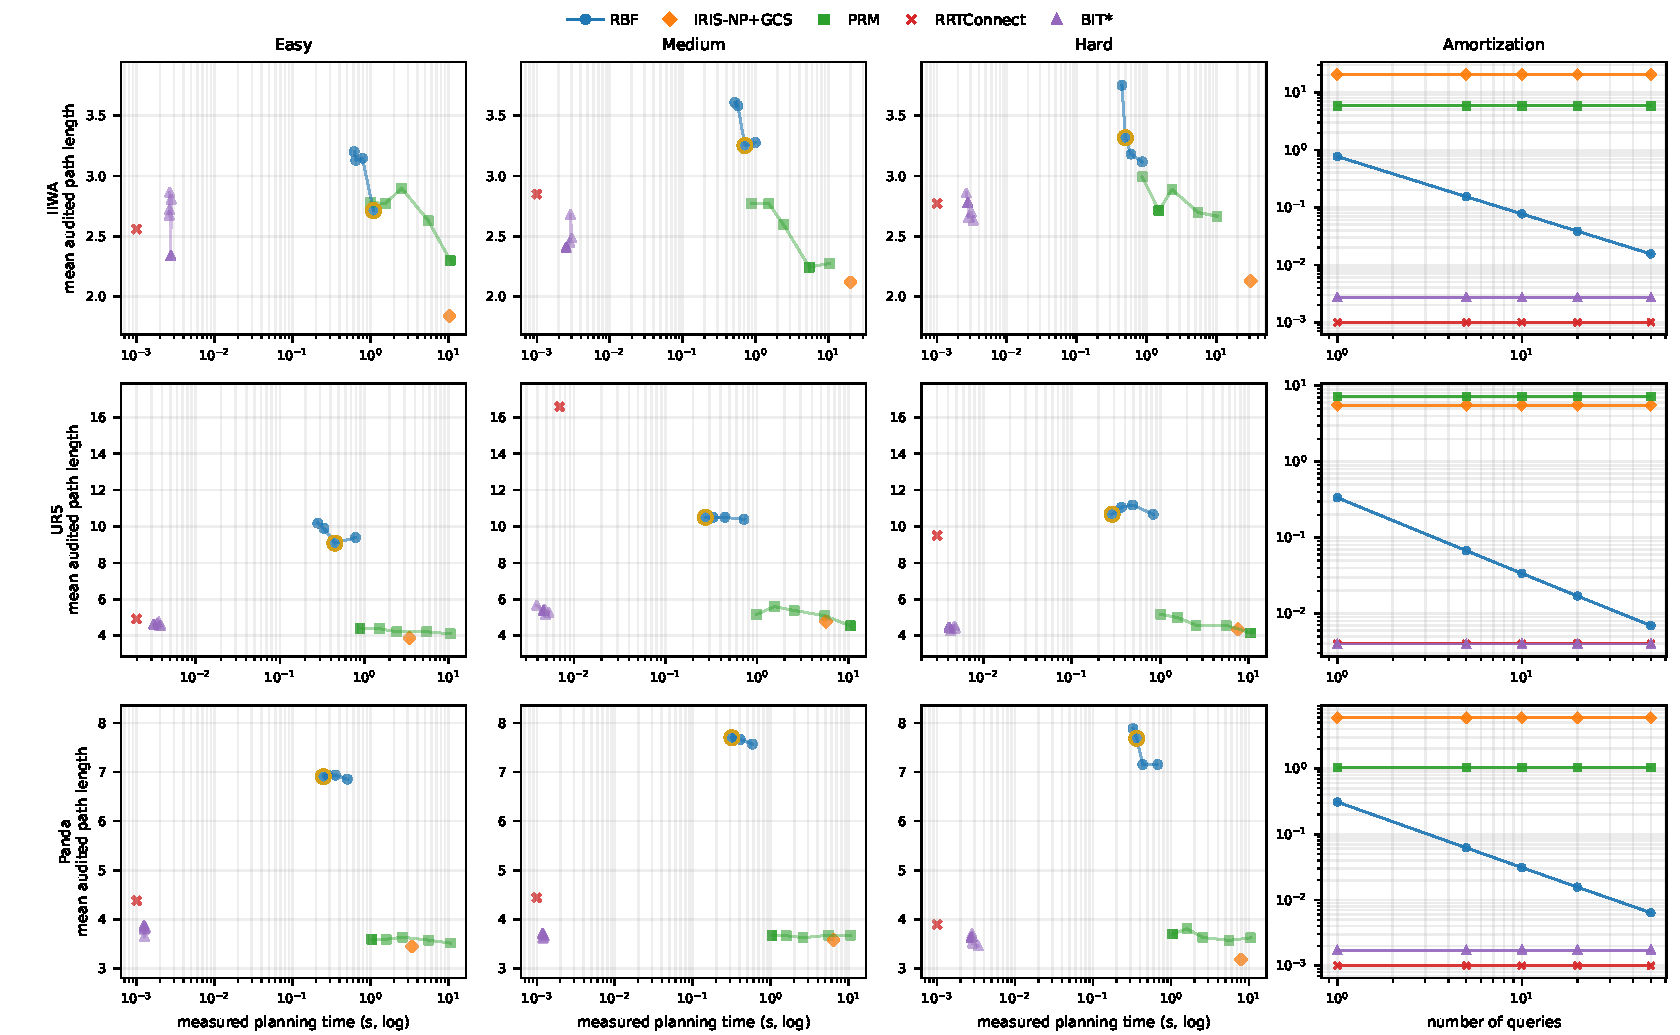
\includegraphics[width=0.84\textwidth,keepaspectratio]{generated/fig_tro_random_tradeoff.pdf}
  \caption{Saved-catalog random-scene trade-off. Left/middle: fixed five-query
  point Build/5 + \onlineq{}; right: reuse horizon \(K\) in Build/\(K\) +
  \onlineq{}. \onlineq{} is per-query online time, and smaller path-length
  ratios are shorter. Rows are the three robot models. The summary table reports
  $N_{\mathrm{ret}}$ and IRIS/GCS $N_{\mathrm{full}}/6$ coverage; no-build
  methods plot at \onlineq{} under the common 8-thread policy. Rings mark first
  validated checkpoints (black) and later \(\ge 1\%\) path-ratio gains (gold);
  PRM and BIT* use offline checkpoints.}
  \label{fig:tro_random_tradeoff}
\end{figure*}

\begin{table*}[!t]
\centering
\TableFontRestore
\begin{table}[t]
\centering
\caption{Endpoint AABB source comparison at fixed joint-box widths. Cert. marks certificate-backed sources. MC uses width-density sampling, and Max neg. gap reports the worst per-axis shortfall against the CritSample/Analytical/MC sampling-union reference.}
\label{tab:tro-endpoint-envelope}
\scriptsize
\setlength{\tabcolsep}{2.0pt}
\renewcommand{\arraystretch}{0.94}
\begin{tabular}{@{}llrrrr@{}}
\toprule
Width & Source & Cert. & $V_{\mathrm{ep}}$ (m$^3$) & Time ($\mu$s) & Max neg. gap \\
\midrule
0.02 & IFK\_AA & Y & 0.000045 & 5.5 & -0.0000 \\
0.02 & HIFK\_3 & Y & 0.000042 & 25.9 & -0.0000 \\
0.02 & HIFK\_5 & Y & 0.000042 & 70.4 & -0.0000 \\
0.02 & CritSample & N & 0.000041 & 8.7 & -0.0000 \\
0.02 & Analytical & Y & 0.000041 & 6430.0 & -0.0000 \\
0.02 & MC & N & 0.000026 & 2251.7 & -0.0061 \\
\addlinespace
0.05 & IFK\_AA & Y & 0.000797 & 6.1 & -0.0000 \\
0.05 & HIFK\_3 & Y & 0.000714 & 26.9 & -0.0000 \\
0.05 & HIFK\_5 & Y & 0.000690 & 71.7 & -0.0000 \\
0.05 & CritSample & N & 0.000647 & 9.0 & -0.0003 \\
0.05 & Analytical & Y & 0.000647 & 6500.4 & -0.0000 \\
0.05 & MC & N & 0.000454 & 5629.2 & -0.0146 \\
\addlinespace
0.10 & IFK\_AA & Y & 0.007709 & 6.5 & -0.0000 \\
0.10 & HIFK\_3 & Y & 0.006187 & 29.2 & -0.0000 \\
0.10 & HIFK\_5 & Y & 0.005748 & 73.8 & -0.0000 \\
0.10 & CritSample & N & 0.005085 & 10.0 & -0.0012 \\
0.10 & Analytical & Y & 0.005086 & 6602.3 & -0.0000 \\
0.10 & MC & N & 0.003739 & 11233.3 & -0.0327 \\
\addlinespace
0.20 & IFK\_AA & Y & 0.095828 & 6.6 & -0.0000 \\
0.20 & HIFK\_3 & Y & 0.063170 & 27.2 & -0.0000 \\
0.20 & HIFK\_5 & Y & 0.054478 & 73.1 & -0.0000 \\
0.20 & CritSample & N & 0.041680 & 11.6 & -0.0045 \\
0.20 & Analytical & Y & 0.041748 & 6800.1 & -0.0000 \\
0.20 & MC & N & 0.032592 & 22353.0 & -0.0656 \\
\addlinespace
0.30 & IFK\_AA & Y & 0.501814 & 6.8 & -0.0000 \\
0.30 & HIFK\_3 & Y & 0.268384 & 29.3 & -0.0000 \\
0.30 & HIFK\_5 & Y & 0.214676 & 75.9 & -0.0000 \\
0.30 & CritSample & N & 0.141227 & 12.7 & -0.0108 \\
0.30 & Analytical & Y & 0.142112 & 6927.1 & -0.0000 \\
0.30 & MC & N & 0.112648 & 33813.6 & -0.0889 \\
\addlinespace
0.50 & IFK\_AA & Y & 5.602815 & 7.4 & -0.0000 \\
0.50 & HIFK\_3 & Y & 2.028027 & 29.4 & -0.0000 \\
0.50 & HIFK\_5 & Y & 1.347150 & 72.3 & -0.0000 \\
0.50 & CritSample & N & 0.639900 & 16.3 & -0.0310 \\
0.50 & Analytical & Y & 0.650907 & 7096.0 & -0.0045 \\
0.50 & MC & N & 0.534496 & 56835.6 & -0.1235 \\
\bottomrule
\end{tabular}
\end{table}

\vspace{0.45ex}
\begin{table}[t]
\centering
\caption{Width-wise IFK\_AA link-envelope comparison with one link split ($S=1$). Entries are means over fixed-width boxes. Env. reports envelope materialization only; Coll. is the standalone obstacle test.}
\label{tab:tro-link-envelope}
\scriptsize
\setlength{\tabcolsep}{2.0pt}
\renewcommand{\arraystretch}{0.94}
\begin{tabular}{@{}llrrr@{}}
\toprule
Width & Envelope & $V$ (m$^3$) & \shortstack{Env.\\($\mu$s)} & \shortstack{Coll.\\($\mu$s)} \\
\midrule
0.02 & LinkIAABB & 0.013628 & 0.1 & 0.3 \\
0.02 & SupportHull & 0.000359 & 0.2 & 2.0 \\
\addlinespace
0.05 & LinkIAABB & 0.020148 & 0.1 & 0.4 \\
0.05 & SupportHull & 0.002662 & 0.2 & 2.1 \\
\addlinespace
0.10 & LinkIAABB & 0.038415 & 0.2 & 0.3 \\
0.10 & SupportHull & 0.014329 & 0.2 & 2.4 \\
\addlinespace
0.20 & LinkIAABB & 0.146513 & 0.1 & 0.4 \\
0.20 & SupportHull & 0.105919 & 0.2 & 3.2 \\
\addlinespace
0.30 & LinkIAABB & 0.507549 & 0.2 & 0.4 \\
0.30 & SupportHull & 0.448860 & 0.2 & 5.2 \\
\addlinespace
0.50 & LinkIAABB & 4.607121 & 0.2 & 0.3 \\
0.50 & SupportHull & 4.537899 & 0.2 & 11.2 \\
\bottomrule
\end{tabular}
\end{table}

\end{table*}

\emph{Dataset and pruning.}
Each saved random scene has ten pre-generated queries shared by every method.
Across KUKA LBR iiwa, Universal Robots UR5, and Franka Emika Panda, the medium
and hard catalogs over ten seeds contain 600 query instances before applying the
fixed, method-independent pruning rule. For each robot and seed, medium and hard
rows share the saved start--goal set; hard rows append a saved obstacle-prefix
extension to the medium row, so difficulty changes are nested rather than
regenerated. Before summarizing any method, the pruning rule removes cases where
the direct start--goal segment already validates without planning. The retained
post-pruning count, denoted $N_{\mathrm{ret}}$, is reported with each
robot/difficulty row in the random-summary table. All methods in a row share
that retained set. The same table carries the IRIS/GCS full-success coverage
field, so baseline coverage is visible without computing medians over
method-specific survivors. The pruning changes summary statistics but not the
saved catalogs, which retain ten queries per scene.

\emph{Compared methods and accounting.}
The trade-off plot uses the five-query amortized quantity Build/5 + \onlineq{}
for rows with reusable builds and \onlineq{} otherwise as a fixed display point;
\(K\) is a reuse horizon, not a post-pruning retained-query count.
Table~\ref{tab:tro-random-summary} and Fig.~\ref{fig:tro_random_tradeoff}
summarize the operating points and corresponding checkpoint curves. \rbf{} builds
one query-agnostic forest per scene and reuses it for the saved query set;
medians are computed over retained post-pruning queries. Random-scene \rbf{}
rows use LECT caches and anchors tied to each robot rather than
Shelf-specific assets. Each \rbf{} row uses the OBB-corridor profile and passes
fixed-step validation on the summarized query set. In those rows, accepted
paths use only converted finite-cover \cspace{} OBB-corridor repair witnesses;
no residual non-corridor segments remain. PRM is built once per scene, whereas
\mbox{RRT-Connect} and BIT* are invoked independently for each query; all OMPL
rows follow the common 8-thread execution policy specified in the protocol.
IRIS/GCS did not satisfy the full validated-success criterion required for
comparable random-scene median \onlineq{} and path-length-ratio rows under the
fixed saved-catalog protocol. The random-summary table therefore reports
$N_{\mathrm{full}}/6$, where $N_{\mathrm{full}}$ is the number of
robot/difficulty rows satisfying that rule, rather than a median operating point;
medians over a method-specific surviving subset are intentionally not reported.
Compact random-scene rows without audit-cost fields are planner-time rows rather
than total accepted-path latency rows.

\emph{Results.}
\mbox{RRT-Connect} has the lowest median \onlineq{} in five of the six operating
points; in Panda-Hard, \rbf{} has the lowest median \onlineq{}. After fixed-step
validation, the \mbox{RRT-Connect} median validated path-length ratio exceeds
the \rbf{} ratio in all six points. With scene-forest reuse, \rbf{} has lower
median \onlineq{} than BIT* in all six points; \(L/\Lrefq{}\) matches
BIT* to table precision in the two IIWA rows and is higher than BIT* in the four
UR5/Panda rows.

\noindent\emph{Takeaway.}
The random catalogs support the intended role of \rbf{}: reusable volumetric
structure improves online time relative to BIT* while producing shorter
validated paths than \mbox{RRT-Connect}. This is not a fastest-single-query
claim, because \mbox{RRT-Connect} remains faster in five of six median \onlineq{}
points.

\subsection{Q4: Mechanism Studies Behind the Default Profile}
\label{sec:exp_mechanisms}

Q4 links the default profile to mechanism measurements rather than end-to-end
planning rows. Tables~\ref{tab:tro-endpoint-envelope}
and~\ref{tab:tro-link-envelope} report joint-interval widths in radians. The
endpoint table separates certificate-capable interval sources (IFK-AA and HIFK)
from reference or filter rows; negative sampled-union gaps indicate finite-sample
undercoverage, not certificate margins.

The link table explains the AABB-first narrow phase. SupportHull/GJK stores
compact support records, but wide boxes can increase GJK calls after broadphase
filtering. Link AABB is coarser, yet its build and hot-loop rejection costs are
lower or comparable in the measured rows. The default profile therefore uses
AABBs for broadphase rejection, interval evidence for conservative claims, and
\Cref{tab:claim_boundary} for non-certificate-backed outputs.

\noindent\emph{Takeaway.}
The default profile uses certificate-capable interval evidence for box-level
claims and a cheap AABB broadphase for hot-loop rejection; all remaining outputs
inherit their status from \Cref{tab:claim_boundary}.

\subsection{Q5: Dynamic-Update Maintenance Cost}
\label{sec:exp_dynamic_updates}

Q5 isolates scene-cache maintenance after obstacle edits. Table~\ref{tab:tro-dynamic-update}
reports cache-maintenance-only timing: its warm-build rows are scene-cache
rebuilds, and no query bridge, connector, simplification, audit, or query timing
is included.
\captionof{table}{Supplementary scene-cache update timings and warm-build/update ratios (outside Q1--Q4)}
\label{tab:tro-dynamic-update}
\scriptsize
\setlength{\tabcolsep}{2.0pt}
\renewcommand{\arraystretch}{0.95}
\begin{tabular}{@{}lcc@{}}
\toprule
Operation & Time (ms) & Warm build/update \\
\midrule
Warm build (10 obstacles) & 922.75 [897.57, 955.67] & -- \\
Insert $10\!\to\!15$ & 6.06 [5.69, 6.54] & 153.3--207.5$\times$ \\
Remove $15\!\to\!10$ & 0.35 [0.31, 1.65] & 943.6--3354.0$\times$ \\
Warm build (15 obstacles) & 958.79 [941.67, 1115.18] & -- \\
\bottomrule
\end{tabular}

This experiment therefore measures how quickly the scene cache updates its
labels and local refill state after obstacle insertions or removals. It is not
an end-to-end post-edit replanning benchmark; query success after an edit
requires the same bridge, repair, simplification, and validation pipeline used
by the planning studies above.

\noindent\emph{Takeaway.}
Maintenance-only rows show cache-update speedups of 153.3--207.5$\times$ for
insertion and 943.6--3354.0$\times$ for removal over a 15-obstacle warm rebuild.
These are cache-maintenance speedups; post-edit planning should be read as the
full query pipeline applied after this lower-cost scene-cache update.

\FloatBarrier
\section{Conclusion}\label{sec:conclusion}

\rbf{} is a reusable scene-construction layer for repeated manipulation queries.
It makes the reused object volumetric and auditable: axis-aligned \cspace{} boxes
are the planning unit, endpoint-to-link swept-capsule bounds are the validation
primitive, and LECT stores kinematics-keyed evidence without importing stale
scene labels. The typed corridor graph records whether a returned path is backed
by conservative boxes or finite-cover OBB corridors, or whether it follows the
validation-required semantics in \Cref{tab:claim_boundary}.

The experiments support the intended middle-ground role. On Shelf+IIWA, d23 LECT
replay reduces median reusable build time from 2.770~s for live HIFK-5 to
0.171~s under the same fixed profile. Across saved random-scene catalogs for
three robot models, \rbf{} is not the fastest per-query method in every case,
but it returns shorter validated paths than RRT-Connect in all six operating
points and lower median \onlineq{} than BIT* in all six. Maintenance-only edit
experiments show cache-update speedups of 153.3--207.5$\times$ for insertion and
943.6--3354.0$\times$ for removal over a 15-obstacle warm rebuild.

\paragraph{Limitations}
First, the certificate model covers active rounded links versus workspace
obstacles; self-collision, attached objects, grippers, task regions, and other
constraints require explicit policy and descriptor support. Second, \onlineq{}
excludes final simplification and post-run validation, and d23 prewarm,
snapshot, and memory costs are outside the online protocol. Third, \rbf{} is
kinematic and collision-centric: dynamic feasibility, time-parameterized
execution, and torque or contact constraints are outside the current claim.
Fourth, \rbf{} is not a complete planner: finite depth, axis-aligned
overapproximation, and finite bridge/repair budgets can miss feasible paths.
These extensions are compatible with the cache-and-policy design, but they
require explicit descriptors and validation policies rather than following from
the present certificates. These limits define the scope of the claim contract in
\Cref{tab:claim_boundary}.

\noindent Within this scope, \rbf{} shows that certificate-aware box-level reuse
can provide a practical middle layer between roadmap reuse and convex-region
optimization for repeated-query manipulation.

\IEEEtriggercmd{\enlargethispage{\baselineskip}}
\IEEEtriggeratref{43}
\bibliographystyle{IEEEtran}
\bibliography{references}

\end{document}
